%% ----------------------------------------------------------------
%% Thesis.tex -- MAIN FILE (the one that you compile with LaTeX)
%% ---------------------------------------------------------------- 

% Set up the document
\documentclass[a4paper, 11pt, twoside, openright]{Thesis}  % Use the "Thesis" style, based on the ECS Thesis style by Steve Gunn
\graphicspath{Figures/}  % Location of the graphics files (set up for graphics to be in PDF format)

% Include any extra LaTeX packages required
\usepackage[square, numbers, comma, sort&compress]{natbib}  % Use the "Natbib" style for the references in the Bibliography
\usepackage{verbatim}  % Needed for the "comment" environment to make LaTeX comments
\usepackage{vector}  % Allows "\bvec{}" and "\buvec{}" for "blackboard" style bold vectors in maths
\hypersetup{urlcolor=blue, colorlinks=true}  % Colours hyperlinks in blue, but this can be distracting if there are many links.

%%Code Systaxis highlited
\usepackage{listings}
\usepackage{color}
\usepackage{textcomp}
\definecolor{listinggray}{gray}{0.9}
\definecolor{lbcolor}{rgb}{0.9,0.9,0.9}
\lstset{
    language=Python,
    basicstyle=\scriptsize,
    upquote=true,
    aboveskip={1.5\baselineskip},
    columns=fullflexible,
    showstringspaces=false,
    extendedchars=true,
    breaklines=true,
    showtabs=false,
    showspaces=false,
    showstringspaces=false,
    identifierstyle=\ttfamily,
    keywordstyle=\color[rgb]{0,0,1},
    commentstyle=\color[rgb]{0.133,0.545,0.133},
    stringstyle=\color[rgb]{0.627,0.126,0.941},
}

\usepackage{hyperref}

\newcommand*{\titleGP}{\begingroup % Create the command for including the title page in the document
\centering % Center all text
\vspace*{\baselineskip} % White space at the top of the page

\rule{\textwidth}{1.6pt}\vspace*{-\baselineskip}\vspace*{2pt} % Thick horizontal line
\rule{\textwidth}{0.4pt}\\[\baselineskip] % Thin horizontal line

{\LARGE DEEP LEARNING STUDY NOTES}\\[0.2\baselineskip] % Title

\rule{\textwidth}{0.4pt}\vspace*{-\baselineskip}\vspace{3.2pt} % Thin horizontal line
\rule{\textwidth}{1.6pt}\\[\baselineskip] % Thick horizontal line

\vfill

\scshape % Small caps
{\Large All credits go to \textbf{L. Fei-Fei, A. Karpathy, J.Johnson} teachers of the CS231n course. Thank you for this amazing course!!}\\[\baselineskip] % Tagline(s) or further description

\vfill

 by \\[\baselineskip]
{\Large Albert Pumarola\par} % Editor list

\endgroup}

%% ----------------------------------------------------------------
\begin{document}

% Include the chapters of the thesis, as separate files
% Just uncomment the lines as you write the chapters


\pagestyle{empty} % Removes page numbers

\titleGP % This command includes the title page

\tableofcontents


\part{DATA}
\chapter{Data Preprocessing}

There are different techniques used in learning in order to improve the accuracy of the model by preprocessing the data:

There are three common forms of data preprocessing a data matrix $X$, where we will assume that $X$ is of size $[N \times D]$ ($N$ is the number of data, $D$ is their dimensionality).

\begin{figure}[!htb]
  \centering
  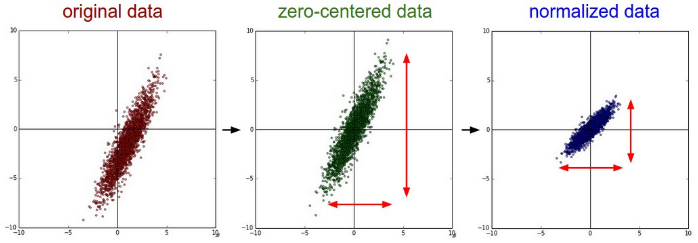
\includegraphics[width=0.7\textwidth]{Images/data_preprocessing/1.png}
  \caption{Preprocessing example 1}
\end{figure}

\begin{figure}[!htb]
  \centering
  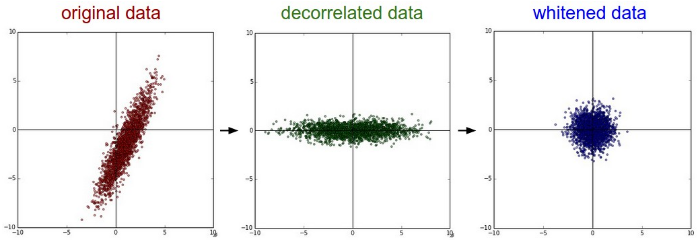
\includegraphics[width=0.7\textwidth]{Images/data_preprocessing/2.png}
  \caption{Preprocessing example 2}
\end{figure}

\paragraph*{Mean subtraction} Most common form of preprocessing. It involves subtracting the mean across every individual feature in the data, and has the geometric interpretation of centring the cloud of data around the origin along every dimension. In NumPy, this operation would be implemented as: \texttt{X -= np.mean(X, axis = 0)}. With images specifically, for convenience it can be common to subtract a single value from all pixels (e.g. \texttt{X -= np.mean(X)}), or to do so separately across the three color channels.

\paragraph*{Normalization} Refers to normalizing the data dimensions so that they are of approximately the same scale. There are two common ways of achieving this normalization. One is to divide each dimension by its standard deviation, once it has been zero-centered: (\texttt{X /= np.std(X, axis = 0)}). Another form of this preprocessing normalizes each dimension so that the min and max along the dimension is -1 and 1 respectively. It only makes sense to apply this preprocessing if you have a reason to believe that different input features have different scales (or units), but they should be of approximately equal importance to the learning algorithm. In case of images, the relative scales of pixels are already approximately equal (and in range from 0 to 255), so it is not strictly necessary to perform this additional preprocessing step.

\paragraph*{PCA} The reason why one would want to use PCA is if one expects that many of the features are in fact dependent. This would be particularly handy for Naive Bayes where independence is assumed. Most datasets are far too large to use PCA. Attention: PCA complexity is $~O(n^3)$, so more sophisticated methods are required. But if your dataset is small, and you don't have the time to investigate more sophisticated methods, then by all means go ahead and apply an out-of-box PCA for feature selection.

\paragraph*{Whitening} Takes the data in the eigenbasis and divides every dimension by the eigenvalue to normalize the scale. The geometric interpretation of this transformation is that if the input data is a multi-variable Gaussian, then the whitened data will be a Gaussian with zero mean and identity covariance matrix.

\subsection*{Deep Learning with images}
For Deep Learning for images we will only use: center our data to zero. To do so, for each pixel, compute its mean across all the dataset and subtract the resulting mean image to all the training samples. If you have more than one channel (e.g. RGB) do it for each of the channels separately.
 
\chapter{Making the most of your data - Data Augmentation and Transfer Learning}

\section{Data Augmentation}

\subsection*{Horizontal Flip} 
\begin{figure}[!htb]
  \centering
  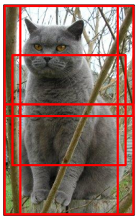
\includegraphics[width=0.125\textwidth]{Images/data_aug_trans/1.png}
  \caption{Horizontal flip. Flip image 180 degrees in the horizontal direction.}
\end{figure}


\subsection*{Random Crops/Scales}
\begin{figure}[!htb]
  \centering
  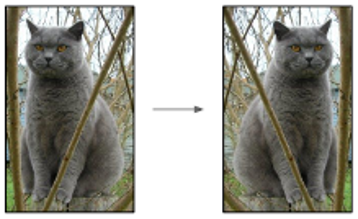
\includegraphics[width=0.3\textwidth]{Images/data_aug_trans/2.png}
  \caption{Random Crops/Scales}
\end{figure}

\textbf{Training}: sample random crops / scales

Specific example. How ResNet trains:
\begin{enumerate}
\item Pick random L in range [256, 480]
\item Resize training image, short side = L
\item Sample random 224 x 224 patch
\end{enumerate}

\textbf{Testing}: average a fixed set of crops 

Specific example. How ResNet tests:
\begin{enumerate}
\item Resize image at 5 scales: {224, 256, 384, 480, 640}
\item For each size, use 10 224 x 224 crops: 4 corners + center, + flips
\end{enumerate}

\subsection*{Color Jitter}
\begin{figure}[!htb]
  \centering
  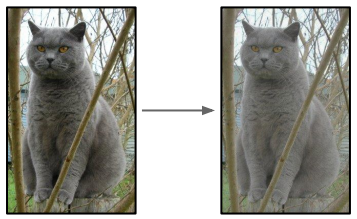
\includegraphics[width=0.3\textwidth]{Images/data_aug_trans/3.png}
  \caption{Color Jitter}
\end{figure}
\begin{itemize}
\item Simple: Randomly jitter contrast

\item Complex:
\begin{enumerate}
\item Apply PCA to all [R, G, B] pixels in training set
\item Sample a “color offset” along principal component directions
\item Add offset to all pixels of a training image
\end{enumerate}
\end{itemize}

\subsection*{Get Creative}
At the end you have to think for your specific case, what transformations you want to be robust to and add them to the training set: translation, 
rotation, stretching, shearing, lens distortions, ...


\section{Transfer Learning}
In practice, very few people train an entire Deep Network from scratch (with random initialization), because it is relatively rare to have a dataset of sufficient size. Instead, it is common to pretrain a ConvNet on a very large dataset (e.g. ImageNet, which contains 1.2 million images with 1000 categories), and then use the ConvNet either as an initialization or a fixed feature extractor for the task of interest. Pretrained DeepNets are usually trained with large computer clusters and downloaded by others. The three major Transfer Learning scenarios look as follows:

\paragraph*{ConvNet as fixed feature extractor} Take a ConvNet pretrained on ImageNet, remove the last fully-connected layer (this layer’s outputs are the 1000 class scores for a different task like ImageNet), then treat the rest of the ConvNet as a fixed feature extractor for the new dataset. In an AlexNet, this would compute a 4096-D vector for every image that contains the activations of the hidden layer immediately before the classifier. We call these features CNN codes. 
\paragraph*{Fine-tuning the ConvNet} The second strategy is not only to replace and retrain the classifier on top of the ConvNet on the new dataset, but to also fine-tune the weights of the pretrained network by continuing the backpropagation. It is possible to fine-tune all the layers of the ConvNet, or it’s possible to keep some of the earlier layers fixed (due to overfitting concerns) and only fine-tune some higher-level portion of the network. This is motivated by the observation that the earlier features of a ConvNet contain more generic features (e.g. edge detectors or color blob detectors) that should be useful to many tasks, but later layers of the ConvNet becomes progressively more specific to the details of the classes contained in the original dataset. In case of ImageNet for example, which contains many dog breeds, a significant portion of the representational power of the ConvNet may be devoted to features that are specific to differentiating between dog breeds.

\paragraph*{Check points of pretrained models} Since modern ConvNets take 2-3 weeks to train across multiple GPUs on ImageNet, it is common to see people release their final ConvNet checkpoints for the benefit of others who can use the networks for fine-tuning. For example, the Caffe library has a Model Zoo where people share their network weights.

\subsection*{When and how to fine-tune?}
\begin{figure}[!htb]
  \centering
  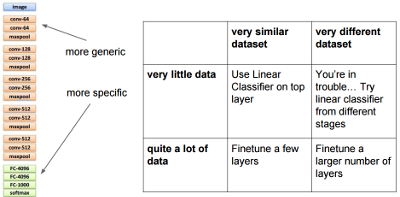
\includegraphics[width=0.6\textwidth]{Images/data_aug_trans/4.png}
  \caption{Random Crops/Scales}
\end{figure}
IMPORTANT: When doing transfer learning if you make changes in the green and orange part do the following:
\begin{itemize}
\item Train green, freeze everything else
\item When green is starting to converge unfreeze the orange part that you want to modify
\end{itemize}

This is necessary because green starts with random values and it may produce very big gradients that may destroy your previous layers

\subsection*{Practical advice}
There are a few additional things to keep in mind when performing Transfer Learning:

\paragraph*{Constraints from pretrained models} Note that if you wish to use a pretrained network, you may be slightly constrained in terms of the architecture you can use for your new dataset. For example, you can’t arbitrarily take out Conv layers from the pretrained network. However, some changes are straight-forward: Due to parameter sharing, you can easily run a pretrained network on images of different spatial size. This is clearly evident in the case of Conv/Pool layers because their forward function is independent of the input volume spatial size (as long as the strides “fit”). In case of FC layers, this still holds true because FC layers can be converted to a Convolutional Layer: For example, in an AlexNet, the final pooling volume before the first FC layer is of size [6x6x512]. Therefore, the FC layer looking at this volume is equivalent to having a Convolutional Layer that has receptive field size 6x6, and is applied with padding of 0.

\paragraph*{Learning rates} It’s common to use a smaller learning rate for ConvNet weights that are being fine-tuned, in comparison to the (randomly-initialized) weights for the new linear classifier that computes the class scores of your new dataset. This is because we expect that the ConvNet weights are relatively good, so we don’t wish to distort them too quickly and too much (especially while the new Linear Classifier above them is being trained from random initialization).

\part{LEARNING}
\chapter{Neural Network}

Imagine a linear classification which computes scores for different visual categories given the image using the formula $s=Wx$, where $W$ is a matrix and $x$ was an input column vector containing all pixel data of the image. In the case of CIFAR-10, $x$ is a $3072 \times 1 $ column vector, and $W$ is a $10 \times 3072$ matrix, so that the output scores is a vector of 10 class scores.

An example neural network would instead compute $s=W_2\max(0,W_1x)$. Here, $W_1$ could be, for example, a $100 \times 3072$ matrix transforming the image into a 100-dimensional intermediate vector. The function $\max(0,−)$ is a non-linearity that is applied elementwise. There are several choices we could make for the non-linearity (which we’ll see later), but this one is a common choice and simply thresholds all activations that are below zero to zero. These are the so called \textit{activation functions}. Finally, the matrix $W_2$ would then be of size $10 \times 100$, so that we again get 10 numbers out that we interpret as the class scores. Notice that the non-linearity is critical computationally - if we left it out, the two matrices could be collapsed to a single matrix, and therefore the predicted class scores would again be a linear function of the input. The non-linearity is where we get the wiggle. The parameters $W_2,W_1$ are learned with stochastic gradient descent, and their gradients are derived with chain rule (and computed with backpropagation).

A three-layer neural network could analogously look like $s=W_3\max(0,W_2\max(0,W_1x))$, where all of $W_3,W_2,W_1$ are parameters to be learned. The sizes of the intermediate hidden vectors are hyperparameters of the network and we’ll see how we can set them later. Lets now look into how we can interpret these computations from the neuron/network perspective.

\begin{figure}[h]
  \centering
  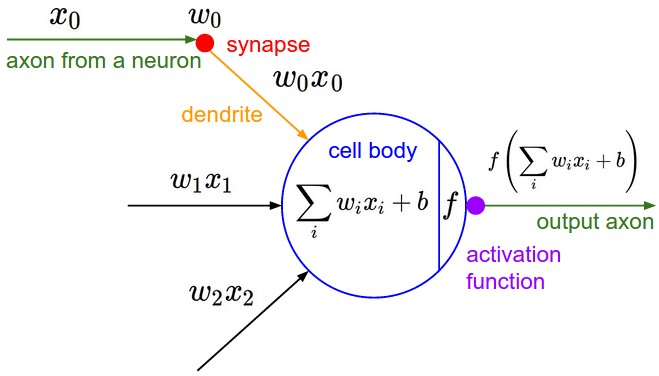
\includegraphics[width=0.4\textwidth]{Images/nn/1.jpeg}
  \caption{Cell diagram}
\end{figure}

An example code for forward-propagating a single neuron might look as follows:


\begin{lstlisting}[frame=single]
class Neuron(object):
  # ... 
  def forward(inputs):
    """ assume inputs and weights are 1-D numpy arrays and bias is a number """
    cell_body_sum = np.sum(inputs * self.weights) + self.bias
    firing_rate = 1.0 / (1.0 + math.exp(-cell_body_sum)) # sigmoid activation function
    return firing_rate
\end{lstlisting}

In other words, each neuron performs a dot product with the input and its weights, adds the bias and applies the non-linearity (or activation function), in this case the sigmoid $\sigma(x)=1/(1+e^{−x})$. We will go into more details about different activation functions at the end of this section.

\subsection*{Single neuron as a linear classifier}

The mathematical form of the model Neuron’s forward computation might look familiar to you. As with linear classifiers, a neuron has the capacity to ``like” (activation near one) or ``dislike” (activation near zero) certain linear regions of its input space. Hence, with an appropriate loss function on the neuron’s output, we can turn a single neuron into a linear classifier:

\paragraph*{Binary Softmax classifier} For example, we can interpret $\sigma(\sum_iw_ix_i+b)$ to be the probability of one of the classes $P(y_i=1∣x_i;w)$. The probability of the other class would be $P(y_i=0∣x_i;w)=1−P(y_i=1∣x_i;w)$, since they must sum to one. With this interpretation, we can formulate the cross-entropy loss as we have seen in the Linear Classification section, and optimizing it would lead to a binary Softmax classifier (also known as logistic regression). Since the sigmoid function is restricted to be between 0-1, the predictions of this classifier are based on whether the output of the neuron is greater than 0.5.

\paragraph*{Binary SVM classifier} Alternatively, we could attach a max-margin hinge loss to the output of the neuron and train it to become a binary Support Vector Machine.

\paragraph*{Regularization interpretation} The regularization loss in both SVM/Softmax cases could in this biological view be interpreted as gradual forgetting, since it would have the effect of driving all synaptic weights $w$ towards zero after every parameter update.

\subsection*{Layer-wise organization}
Neural Networks as neurons in graphs. Neural Networks are modeled as collections of neurons that are connected in an acyclic graph. In other words, the outputs of some neurons can become inputs to other neurons. Cycles are not allowed since that would imply an infinite loop in the forward pass of a network. Instead of an amorphous blobs of connected neurons, Neural Network models are often organized into distinct layers of neurons. For regular neural networks, the most common layer type is the \textbf{fully-connected layer} in which neurons between two adjacent layers are fully pairwise connected, but neurons within a single layer share no connections. 

\begin{figure}[h]
  \centering
  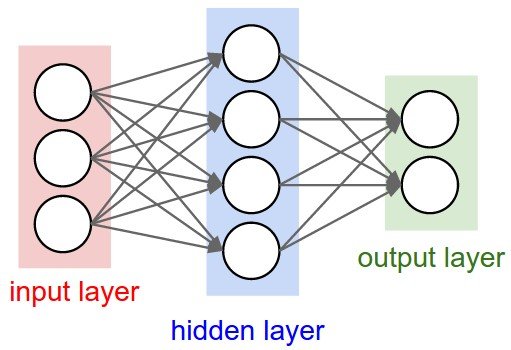
\includegraphics[width=0.3\textwidth]{Images/nn/2.jpeg}
  \caption{Layer-wise organization. A 2-layer Neural Network (one hidden layer of 4 neurons (or units) and one output layer with 2 neurons), and three inputs}
\end{figure}

\subsection*{Example feed-forward computation}
\begin{lstlisting}[frame=single]
# forward-pass of a 3-layer neural network:
f = lambda x: 1.0/(1.0 + np.exp(-x)) # activation function (use sigmoid)
x = np.random.randn(3, 1) # random input vector of three numbers (3x1)
h1 = f(np.dot(W1, x) + b1) # calculate first hidden layer activations (4x1)
h2 = f(np.dot(W2, h1) + b2) # calculate second hidden layer activations (4x1)
out = np.dot(W3, h2) + b3 # output neuron (1x1)
\end{lstlisting}


\subsection*{Setting number of layers and their sizes}
How do we decide on what architecture to use when faced with a practical problem? Should we use no hidden layers? One hidden layer? Two hidden layers? How large should each layer be? First, note that as we increase the size and number of layers in a Neural Network, the capacity of the network increases. That is, the space of representable functions grows since the neurons can collaborate to express many different functions. For example, suppose we had a binary classification problem in two dimensions. We could train three separate neural networks, each with one hidden layer of some size and obtain different classifiers (Fig. \ref{fig:nn_classifiers}).

\begin{figure}[h]
  \centering
  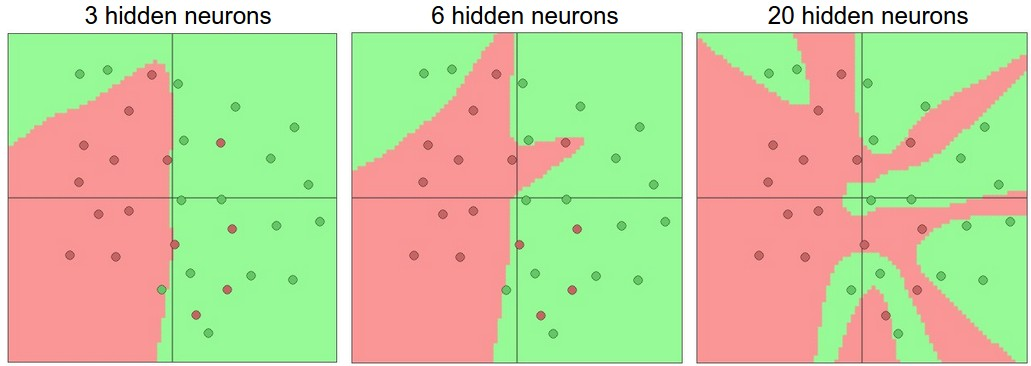
\includegraphics[width=0.6\textwidth]{Images/nn/3.jpeg}
  \caption{Larger Neural Networks can represent more complicated functions. You can play with these examples in \href{http://cs.stanford.edu/people/karpathy/convnetjs/demo/classify2d.html}{this ConvNetsJS demo}.}
  \label{fig:nn_classifiers}
\end{figure}

In the diagram above, we can see that Neural Networks with more neurons can express more complicated functions. However, this is both a blessing (since we can learn to classify more complicated data) and a curse (since it is easier to overfit the training data). \textbf{Overfitting} occurs when a model with high capacity fits the noise in the data instead of the (assumed) underlying relationship. For example, the model with 20 hidden neurons fits all the training data but at the cost of segmenting the space into many disjoint red and green decision regions. The model with 3 hidden neurons only has the representational power to classify the data in broad strokes. It models the data as two blobs and interprets the few red points inside the green cluster as \textbf{outliers} (noise). In practice, this could lead to better \textbf{generalization} on the test set. To reiterate, the \textbf{regularization} strength is the preferred way to control the overfitting of a neural network. We can look at the results achieved by three different settings (Fig. \ref{fig:nn_reg}).

\begin{figure}[h]
  \centering
  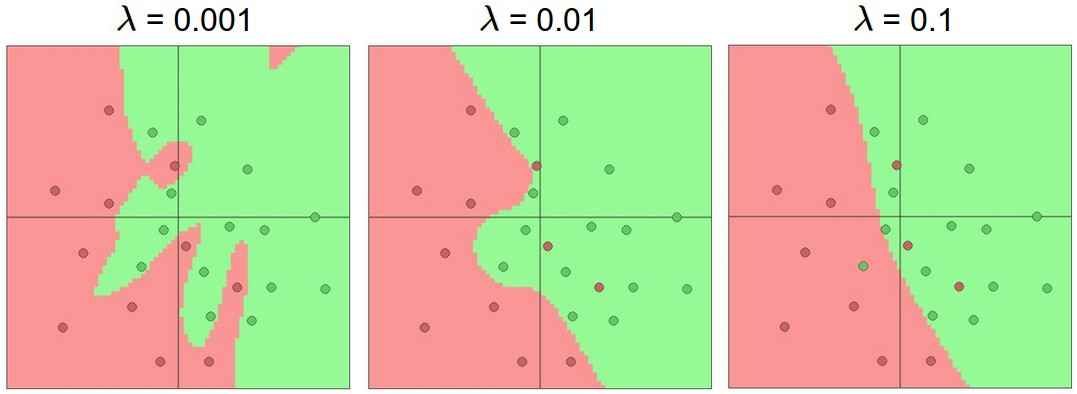
\includegraphics[width=0.6\textwidth]{Images/nn/4.jpeg}
  \caption{The effects of regularization strength: Each neural network above has 20 hidden neurons, but changing the regularization strength makes its final decision regions smoother with a higher regularization. You can play with these examples in \href{http://cs.stanford.edu/people/karpathy/convnetjs/demo/classify2d.html}{this ConvNetsJS demo}.}
    \label{fig:nn_reg}
\end{figure}
\chapter{Parameters Initialization}

\section{Weights}
We normally want the weights to be close to zero because it is reasonable to think that half of the wights will be positive and half of them will be negative.

Warning: It’s not necessarily the case that smaller numbers will work strictly better. For example, a Neural Network layer that has very small weights will during backpropagation compute very small gradients on its data (since this gradient is proportional to the value of the weights). This could greatly diminish the “gradient signal” flowing backward through a network, and could become a concern for deep networks. It would bring all the activations towards 0.

If the weight are initialized with a to high value the activations will explode and saturate to 1.

\subsection*{W=0}
There is no balance break. If every neuron in the network computes the same output, then they will also all compute the same greadients during backpropagation and undergo the exact same parameter updates. In other words, there is no source of asymmetry between neurons if thir weights are initialized to be the same.

\subsection*{Small random numbers}
Every neuron’s weight vector is initialized as a random vector sampled from a multi-dimensional gaussian, so the neurons point in random direction in the input space. It is also possible to use small numbers drawn from a uniform distribution, but this seems to have relatively little impact on the final performance in practice.

One of the problems of this method is to decide how small should the gradients be. Example assuiming tanh:
\begin{itemize}
\item \texttt{W = 0.01 * np.random.randn(D,H)} : might be too small, all activations become zero, therefore, no gradient accumulation.
\item \texttt{W = 1* np.random.randn(D,H)} : might be too large, almost all neurons completely saturated, thus gradients will be zero.
\end{itemize}

Another problem is that the distribution of the outputs from a randomly initialized neuron has a variance that grows with the number of inputs.


\subsection*{Xavier initialization}
\textbf{eq}: \texttt{w = np.random.randn(n) / sqrt(n)}

\textbf{eq for ReLU}: \texttt{w = np.random.randn(n) / sqrt(2n)}

It is possible to solve the distribution problem of the above method by normalizing the variance of each neuron’s output to 1 by scaling its weight vector by the square root of its fan-in (i.e. its number of inputs). This ensures that all neurons in the network initially have approximately the same output distribution and empirically improves the rate of convergence.

\subsubsection*{Mathematical reasoning}
Consider the inner product $s=\sum_i^n w_ix_i$ between the weights  and input , which gives the raw activation of a neuron before the non-linearity. We can examine the variance of $s$:

\begin{equation}
\begin{aligned}
\text{Var}(s) &= \text{Var}(\sum_i^n w_ix_i) \\
& =  \sum_i^n \text{Var}(w_ix_i)\\
& = \sum_i^n [E(w_i)]^2\text{Var}(x_i)+\text{E}[(x_i)]^2\text{Var}(w_i)+\text{Var}(x_i)\text{Var}(w_i)\\
& = \sum_i^n \text{Var}(x_i)\text{Var}(w_i)\\
& = (n\text{Var}(w))\text{Var}(x)\\
\end{aligned}
\end{equation}

where in the first 2 steps we have used properties of variance. In third step we assumed zero mean inputs and weights, so $E[x_i] = E[w_i] = 0$. Note that this is not generally the case: For example ReLU units will have a positive mean. In the last step we assumed that all $x_i,w_i$ are identically distributed. From this derivation we can see that if we want $s$ to have the same variance as all of its inputs $xx$, then during initialization we should make sure that the variance of every weight $w$ is $1/n$. And since $\text{Var}(aX) = a^2\text{Var}(X)$ for a random variable $X$ and a scalar $a$, this implies that we should draw from unit Gaussian and then scale it by $a = \sqrt{1/n}$, to make its variance $1/n$. This gives the initialization \texttt{w = np.random.randn(n) / sqrt(n)}.

A similar analysis is carried out for ReLUs, reaching the conclusion that the variance of neurons in the network should be . This gives the initialization \texttt{w = np.random.randn(n) / sqrt(2n)}, and is the current recommendation for use in practice in the specific case of neural networks with ReLU neurons.

\subsection*{Sparse Initialization}
Another way to address the uncalibrated variances problem is to set all weight matrices to zero, but to break symmetry every neuron is randomly connected (with weights sampled from a small gaussian as above) to a fixed number of neurons below it. A typical number of neurons to connect to may be as small as 10.

\section{Biases}
It is possible and common to initialize the biases to be zero, since the asymmetry breaking is provided by the small random numbers in the weights. For ReLU non-linearities, some people like to use small constant value such as 0.01 for all biases because this ensures that all ReLU units fire in the beginning and therefore obtain and propagate some gradient. However, it is not clear if this provides a consistent improvement (in fact some results seem to indicate that this performs worse) and it is more common to simply use 0 bias initialization.

\section*{Summary}
The current recommendation is to use ReLU units and use the Xavier initialization \texttt{w = np.random.randn(n) * sqrt(2.0/n)} and all biases equal to 0 or ~0.01. Also batch normalization helps having less headaches with weight initialization.
\chapter{Activation Function}

Activation functions are needed in order to increase the complexity of the NN, without them it would just be a linear sandwich of linear functions (multiplying linear functions = linear function)


\section{Sigmoid}

\begin{figure}[!htb]
  \centering
  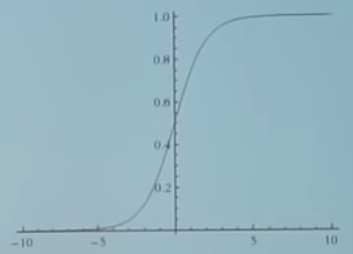
\includegraphics[width=0.3\textwidth]{Images/activation_f/1.png}
  \caption{Sigmoid }
\end{figure}
$\sigma (x) = \frac{1}{1+e^{-x}}$
\begin{itemize}
\item \textcolor{red}{Saturated neurons "kill" the gradient}
\item \textcolor{red}{No zero-centered output}
\item \textcolor{red}{exp() is computationaly expensive}
\end{itemize}


\section{Tanh}
\begin{figure}[!htb]
  \centering
  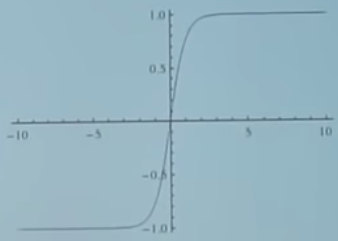
\includegraphics[width=0.3\textwidth]{Images/activation_f/2.png}
  \caption{Tanh }
\end{figure}
$\text{tanh} (x) = \frac{2}{e^{-2x}+1}-1$
\begin{itemize}
\item \textcolor{green}{Zero centered output}
\item \textcolor{red}{Saturated neurons "kill" the gradient}
\end{itemize}


\section{ReLU}
\begin{figure}[!htb]
  \centering
  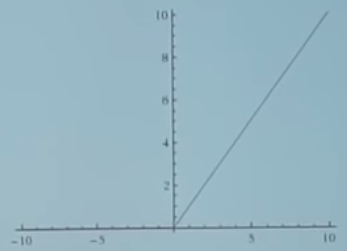
\includegraphics[width=0.3\textwidth]{Images/activation_f/3.png}
  \caption{ReLU }
\end{figure}
$f(x) = \max(0,x)$ If a neuron has $x < 0$ the ReLU kills it in backprop. The gradient will be 0 so that neuron will not backprop downwards and its weights will not be updated. Its like a boolean gate. The gradient in the case of $x=0$ is undefined (unlike case).

\begin{itemize}
\item \textcolor{green}{Does not saturate}
\item \textcolor{green}{Computationally efficient}
\item \textcolor{green}{Converges mch faster than sigmoid/tanh in practive ($~6x$)}

\item \textcolor{red}{Not zero centred output}
\item \textcolor{red}{If your unlucky a neuron may be never active because the initialization has put it outside the manifold.}
\item \textcolor{red}{When the learning rate is high is easy to kill a lot of neurons. Imagine the activation function as a threshold which is moving while training. If the learning rate is to high it may move out of the data manifold. In that case the neuron dies and will never be able to recover because will never update again.}
\end{itemize}

It is a good practice to initialize them with a slightly positive initial bias to avoid "dead neurons"

\section{Leaky ReLU}
\begin{figure}[h]
  \centering
  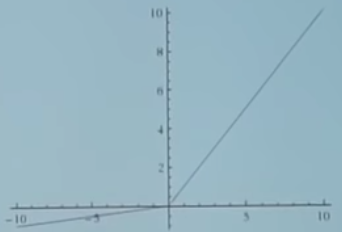
\includegraphics[width=0.3\textwidth]{Images/activation_f/5.png}
  \caption{Leaky ReLU}
\end{figure}
$f(x) = \max(\alpha x,x) = \left\{\begin{matrix}
\alpha x & \text{if}(x\leq 0)\\ 
x & \text{if}(x>  0)
\end{matrix}\right.$
where  $\alpha$ is a very small number $~0.01$ which can be a hyperparameter or learned through .

\begin{itemize}
\item \textcolor{green}{Does not saturate}
\item \textcolor{green}{Computationally efficient}
\item \textcolor{green}{Converges much faster than sigmoid/tanh in practice ($~6x$)}
\item \textcolor{green}{Does not die}

\item \textcolor{red}{Not zero centred output}
\item \textcolor{red}{Consistency of the benefits across tasks not clear}
\end{itemize}

\section{ELU - Exponential Linear Units}

\begin{figure}[!htb]
  \centering
  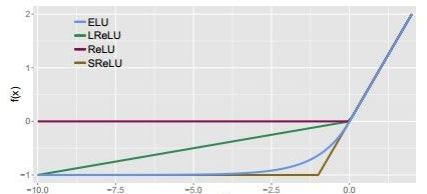
\includegraphics[width=0.5\textwidth]{Images/activation_f/6.png}
  \caption{ELU}
\end{figure}
$f(x) = \left\{\begin{matrix}
\alpha(e^x-1) & \text{if}(x\leq 0)\\ 
x & \text{if}(x>  0)
\end{matrix}\right.$
\begin{itemize}
\item \textcolor{green}{All benefits of ReLu}
\item \textcolor{green}{Does not die}
\item \textcolor{green}{Closer to zero mean outputs}

\item \textcolor{red}{exp() is computationally expensive}
\item \textcolor{red}{There is controversy if it actually trains better with this than with ReLU}
\end{itemize}

\section{Maxout}

\begin{figure}[!htb]
  \centering
  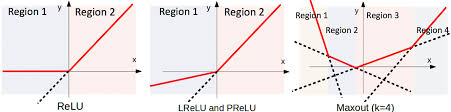
\includegraphics[width=0.6\textwidth]{Images/activation_f/7.jpg}
  \caption{Maxout}
\end{figure}
$f(x) = \max(w_1^Tx+b_1,w_2^Tx+b_2)$
\begin{itemize}
\item \textcolor{green}{Generalized ReLU and Leaky ReLU}
\item \textcolor{green}{Does not saturate}
\item \textcolor{green}{Does not die}
\item \textcolor{green}{Linear Regime}

\item \textcolor{red}{Doubles the number of parameters/neuros}
\end{itemize}

\section*{Conclusion}
\begin{itemize}
\item \textbf{Use ReLU} but be careful with your learning rates. So for example a 3-layer neural network will look like this:
\item Try out Leaky ReLU/Maxout/ELU
\item Try out tanh but don't expect much
\item Don't use sigmoid
\end{itemize}

\chapter{Loss function}

We have discussed the regularization loss part of the objective, which can be seen as penalizing some measure of complexity of the model. The second part of an objective is the data loss, which in a supervised learning problem measures the compatibility between a prediction (e.g. the class scores in classification) and the ground truth label. The data loss takes the form of an average over the data losses for every individual example. That is, $L = \frac{1}{N} \sum_i L_i$ where $N$ is the number of training data. Lets abbreviate $f = f(x_i; W)$ to be the activations of the output layer in a Neural Network. There are several types of problems you might want to solve in practice:

\section*{Classification}

Classification is the case that we have so far discussed at length. Here, we assume a dataset of examples and a single correct label (out of a fixed set) for each example. One of two most commonly seen cost functions in this setting are the SVM (e.g. the Weston Watkins formulation):

\begin{equation}
L_i = \sum_{j\neq y_i} \max(0, f_j - f_{y_i} + 1)
\end{equation}

As we briefly alluded to, some people report better performance with the squared hinge loss (i.e. instead using $\max(0, f_j - f_{y_i} + 1)^2$). The second common choice is the Softmax classifier that uses the cross-entropy loss:

\begin{equation}
L_i = -\log\left(\frac{e^{f_{y_i}}}{ \sum_j e^{f_j} }\right)
\end{equation}

In some rough sense, the cross-entropy is measuring how inefficient our predictions are for describing the truth.

\textit{Noise-contrastive estimation} is a sampling loss typically used to train classifiers with a large output vocabulary. Calculating the softmax over a large number of possible classes is prohibitively expensive. Using NCE, we can reduce the problem to binary classification problem by training the classifier to discriminate between samples from the “real” distribution and an artificially generated noise distribution.

\subsection*{Problem}

Large number of classes. When the set of labels is very large (e.g. words in English dictionary, or ImageNet which contains 22,000 categories), it may be helpful to use Hierarchical Softmax. The hierarchical softmax decomposes labels into a tree. Each label is then represented as a path along the tree, and a Softmax classifier is trained at every node of the tree to disambiguate between the left and right branch. The structure of the tree strongly impacts the performance and is generally problem-dependent.

\section*{Attribute Classification}
Both losses above assume that there is a single correct answer $y_i$. But what if $y_i$ is a binary vector where every example may or may not have a certain attribute, and where the attributes are not exclusive? For example, images on Instagram can be thought of as labeled with a certain subset of hashtags from a large set of all hashtags, and an image may contain multiple. A sensible approach in this case is to build a binary classifier for every single attribute independently. For example, a binary classifier for each category independently would take the form:

\begin{equation}
L_i = \sum_j \max(0, 1 - y_{ij} f_j)
\end{equation}

where the sum is over all categories $j$, and $y_{ij}$ is either +1 or -1 depending on whether the i-th example is labeled with the j-th attribute, and the score vector $f_j$ will be positive when the class is predicted to be present and negative otherwise. Notice that loss is accumulated if a positive example has score less than +1, or when a negative example has score greater than -1.

An alternative to this loss would be to train a logistic regression classifier for every attribute independently. A binary logistic regression classifier has only two classes (0,1), and calculates the probability of class 1 as:

\begin{equation}
P(y = 1 \mid x; w, b) = \frac{1}{1 + e^{-(w^Tx +b)}} = \sigma (w^Tx + b)
\end{equation}

Since the probabilities of class 1 and 0 sum to one, the probability for class 0 is $P(y = 0 \mid x; w, b) = 1 - P(y = 1 \mid x; w,b)$. Hence, an example is classified as a positive example (y = 1) if $\sigma (w^Tx + b) > 0.5$, or equivalently if the score $w^Tx +b > 0$. The loss function then maximizes the log likelihood of this probability. You can convince yourself that this simplifies to:

\begin{equation}
L_i = \sum_j y_{ij} \log(\sigma(f_j)) + (1 - y_{ij}) \log(1 - \sigma(f_j))
\end{equation}

where the labels $y_{ij}$ are assumed to be either 1 (positive) or 0 (negative), and $\sigma(\cdot)$ is the sigmoid function. The expression above can look scary but the gradient on $f$ is in fact extremely simple and intuitive: $\partial{L_i} / \partial{f_j} = y_{ij} - \sigma(f_j)$ (as you can double check yourself by taking the derivatives).

\section*{Regression}
Regression is the task of predicting real-valued quantities, such as the price of houses or the length of something in an image. For this task, it is common to compute the loss between the predicted quantity and the true answer and then measure the L2 squared norm, or L1 norm of the difference. The L2 norm squared would compute the loss for a single example of the form:

\begin{equation}
L_i = \Vert f - y_i \Vert_2^2
\end{equation}

The reason the L2 norm is squared in the objective is that the gradient becomes much simpler, without changing the optimal parameters since squaring is a monotonic operation. The L1 norm would be formulated by summing the absolute value along each dimension:

\begin{equation}
L_i = \Vert f - y_i \Vert_1 = \sum_j \mid f_j - (y_i)_j \mid
\end{equation}

where the sum $\sum_j$ is a sum over all dimensions of the desired prediction, if there is more than one quantity being predicted. Looking at only the j-th dimension of the i-th example and denoting the difference between the true and the predicted value by $\delta_{ij}$, the gradient for this dimension (i.e. $\partial{L_i} / \partial{f_j}$ is easily derived to be either $\delta_{ij}$ with the L2 norm, or $sign(\delta_{ij})$. That is, the gradient on the score will either be directly proportional to the difference in the error, or it will be fixed and only inherit the sign of the difference.

\paragraph*{Outliers} L2 norm is not that good dealing with outliers in the training samples. You may consider L1 or variations of L2.

\paragraph*{Word of caution} It is important to note that the L2 loss is much harder to optimize than a more stable loss such as Softmax. Intuitively, it requires a very fragile and specific property from the network to output exactly one correct value for each input (and its augmentations). Notice that this is not the case with Softmax, where the precise value of each score is less important: It only matters that their magnitudes are appropriate. Additionally, the L2 loss is less robust because outliers can introduce huge gradients. When faced with a regression problem, first consider if it is absolutely inadequate to quantize the output into bins. For example, if you are predicting star rating for a product, it might work much better to use 5 independent classifiers for ratings of 1-5 stars instead of a regression loss. Classification has the additional benefit that it can give you a distribution over the regression outputs, not just a single output with no indication of its confidence. If you’re certain that classification is not appropriate, use the L2 but be careful: For example, the L2 is more fragile and applying dropout in the network (especially in the layer right before the L2 loss) is not a great idea.

When faced with a regression task, first consider if it is absolutely necessary. Instead, have a strong preference to discretizing your outputs to bins and perform classification over them whenever possible.

\section*{Structured prediction}
The structured loss refers to a case where the labels can be arbitrary structures such as graphs, trees, or other complex objects. Usually it is also assumed that the space of structures is very large and not easily enumerable. The basic idea behind the structured SVM loss is to demand a margin between the correct structure $yi$ and the highest-scoring incorrect structure. It is not common to solve this problem as a simple unconstrained optimization problem with gradient descent. Instead, special solvers are usually devised so that the specific simplifying assumptions of the structure space can be taken advantage of. We mention the problem briefly but consider the specifics to be outside of the scope of the class.
\chapter{Backpropagation}

\section*{Introduction}

\paragraph*{Motivation} In this section we will develop expertise with an intuitive understanding of backpropagation, which is a way of computing gradients of expressions through recursive application of \textbf{chain rule}. Understanding of this process and its subtleties is critical for you to understand, and effectively develop, design and debug Neural Networks.

\paragraph*{Problem statement} The core problem studied in this section is as follows: We are given some function $f(x)$ where $x$ is a vector of inputs and we are interested in computing the gradient of $f$ at $x$ (i.e. $\nabla f(x)$ ).

\paragraph*{Motivation} Recall that the primary reason we are interested in this problem is that in the specific case of Neural Networks, $f$ will correspond to the loss function ( $L$ ) and the inputs $x$ will consist of the training data and the neural network weights. For example, the loss could be the SVM loss function and the inputs are both the training data $(x_i,y_i), i=1 \ldots N$ and the weights and biases $W,b$. Note that (as is usually the case in Machine Learning) we think of the training data as given and fixed, and of the weights as variables we have control over. Hence, even though we can easily use backpropagation to compute the gradient on the input examples $x_i$, in practice we usually only compute the gradient for the parameters (e.g. $W,b$) so that we can use it to perform a parameter update. However, as we will see later in the class the gradient on xixi can still be useful sometimes, for example for purposes of visualization and interpreting what the Neural Network might be doing.

If you are coming to this class and you’re comfortable with deriving gradients with chain rule, we would still like to encourage you to at least skim this section, since it presents a rarely developed view of backpropagation as backward flow in real-valued circuits and any insights you’ll gain may help you throughout the class.


\section*{Simple expressions and interpretation of the gradient}

Lets start simple so that we can develop the notation and conventions for more complex expressions. Consider a simple multiplication function of two numbers $f(x,y)=xy$. It is a matter of simple calculus to derive the partial derivative for either input:

\begin{equation}
f(x,y) = x y \hspace{0.5in} \rightarrow \hspace{0.5in} \frac{\partial f}{\partial x} = y \hspace{0.5in} \frac{\partial f}{\partial y} = x
\end{equation}

\paragraph*{Interpretation} Keep in mind what the derivatives tell you: They indicate the rate of change of a function with respect to that variable surrounding an infinitesimally small region near a particular point:
\begin{equation}
\frac{df(x)}{dx} = \lim_{h\ \to 0} \frac{f(x + h) - f(x)}{h}
\end{equation}
A technical note is that the division sign on the left-hand sign is, unlike the division sign on the right-hand sign, not a division. Instead, this notation indicates that the operator $\frac{d}{dx}$ is being applied to the function $f$, and returns a different function (the derivative). A nice way to think about the expression above is that when hh is very small, then the function is well-approximated by a straight line, and the derivative is its slope. In other words, the derivative on each variable tells you the sensitivity of the whole expression on its value. For example, if $x=4,y=−3$ then $f(x,y)=−12$ and the derivative on $x$ $\frac{\partial f}{\partial x} = -3$. This tells us that if we were to increase the value of this variable by a tiny amount, the effect on the whole expression would be to decrease it (due to the negative sign), and by three times that amount. This can be seen by rearranging the above equation ( $f(x + h) = f(x) + h \frac{df(x)}{dx}$ ). Analogously, since $\frac{\partial f}{\partial y} = 4$, we expect that increasing the value of $y$ by some very small amount $h$ would also increase the output of the function (due to the positive sign), and by $4h$.

The derivative on each variable tells you the sensitivity of the whole expression on its value.

As mentioned, the gradient $\nabla f$ is the vector of partial derivatives, so we have that $\nabla f = [\frac{\partial f}{\partial x}, \frac{\partial f}{\partial y}] = [y, x]$. Even though the gradient is technically a vector, we will often use terms such as ``the gradient on x” instead of the technically correct phrase ``the partial derivative on x” for simplicity.

We can also derive the derivatives for the addition operation:

\begin{equation}
f(x,y) = x + y \hspace{0.5in} \rightarrow \hspace{0.5in} \frac{\partial f}{\partial x} = 1 \hspace{0.5in} \frac{\partial f}{\partial y} = 1
\end{equation}

that is, the derivative on both $x,y$ is one regardless of what the values of $x,y$ are. This makes sense, since increasing either $x,y$ would increase the output of $f$, and the rate of that increase would be independent of what the actual values of $x,y$ are (unlike the case of multiplication above). The last function we’ll use quite a bit in the class is the max operation:

\begin{equation}
f(x,y) = \max(x, y) \hspace{0.5in} \rightarrow \hspace{0.5in} \frac{\partial f}{\partial x} = (x >= y) \hspace{0.5in} \frac{\partial f}{\partial y} = (y >= x)
\end{equation}

That is, the (sub)gradient is 1 on the input that was larger and 0 on the other input. Intuitively, if the inputs are $x=4,y=2$, then the max is 4, and the function is not sensitive to the setting of $y$. That is, if we were to increase it by a tiny amount $h$, the function would keep outputting 4, and therefore the gradient is zero: there is no effect. Of course, if we were to change $y$ by a large amount (e.g. larger than 2), then the value of $f$ would change, but the derivatives tell us nothing about the effect of such large changes on the inputs of a function; They are only informative for tiny, infinitesimally small changes on the inputs, as indicated by the $\lim_{h \rightarrow 0}$ in its definition.


\section*{Compound expressions with chain rule}

Lets now start to consider more complicated expressions that involve multiple composed functions, such as $f(x,y,z) = (x + y) z$. This expression is still simple enough to differentiate directly, but we’ll take a particular approach to it that will be helpful with understanding the intuition behind backpropagation. In particular, note that this expression can be broken down into two expressions: $q=x+y$ and $f=qz$. Moreover, we know how to compute the derivatives of both expressions separately, as seen in the previous section. $f$ is just multiplication of $q$ and $z$, so $\frac{\partial f}{\partial q} = z, \frac{\partial f}{\partial z} = q$ and $q$ is addition of $x$ and $y$ so $\frac{\partial q}{\partial x} = 1, \frac{\partial q}{\partial y} = 1$. However, we don’t necessarily care about the gradient on the intermediate value $q$ - the value of $\frac{\partial f}{\partial q}$ is not useful. Instead, we are ultimately interested in the gradient of $f$ with respect to its inputs $x,y,z$. The chain rule tells us that the correct way to ``chain” these gradient expressions together is through multiplication. For example, $\frac{\partial f}{\partial x} = \frac{\partial f}{\partial q} \frac{\partial q}{\partial x}$. In practice this is simply a multiplication of the two numbers that hold the two gradients. Lets see this with an example:

\begin{lstlisting}[frame=single]
# set some inputs
x = -2; y = 5; z = -4

# perform the forward pass
q = x + y # q becomes 3
f = q * z # f becomes -12

# perform the backward pass (backpropagation) in reverse order:
# first backprop through f = q * z
dfdz = q # df/dz = q, so gradient on z becomes 3
dfdq = z # df/dq = z, so gradient on q becomes -4
# now backprop through q = x + y
dfdx = 1.0 * dfdq # dq/dx = 1. And the multiplication here is the chain rule!
dfdy = 1.0 * dfdq # dq/dy = 1
\end{lstlisting}

At the end we are left with the gradient in the variables \texttt{[dfdx,dfdy,dfdz]}, which tell us the sensitivity of the variables \texttt{x,y,z} on \texttt{f}. This is the simplest example of backpropagation. Going forward, we will want to use a more concise notation so that we don’t have to keep writing the \texttt{df} part. That is, for example instead of \texttt{dfdq} we would simply write \texttt{dq}, and always assume that the gradient is with respect to the final output.

\begin{figure}[h]
  \centering
  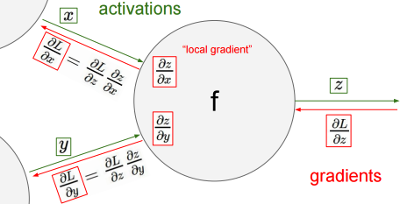
\includegraphics[width=0.5\textwidth]{Images/backprop/1.png}
  \caption{Neuron backprop}
\end{figure}

This computation can also be nicely visualized with a circuit diagram in figure \ref{fig:backdiag1}. The real-valued "circuit" on left shows the visual representation of the computation. The forward pass computes values from inputs to output (shown in green). The backward pass then performs backpropagation which starts at the end and recursively applies the chain rule to compute the gradients (shown in red) all the way to the inputs of the circuit. The gradients can be thought of as flowing backwards through the circuit.

\begin{figure}[h]
  \centering
  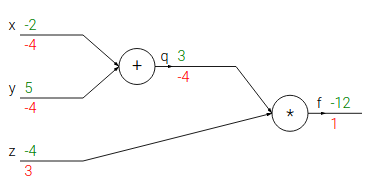
\includegraphics[width=0.5\textwidth]{Images/backprop/2.png}
  \caption{Neuron backprop diagram}
   \label{fig:backdiag1}
\end{figure}

\section*{Intuitive understanding of backpropagation}

Notice that backpropagation is a beautifully local process. Every gate in a circuit diagram gets some inputs and can right away compute two things: 1. its output value and 2. the local gradient of its inputs with respect to its output value. Notice that the gates can do this completely independently without being aware of any of the details of the full circuit that they are embedded in. However, once the forward pass is over, during backpropagation the gate will eventually learn about the gradient of its output value on the final output of the entire circuit. Chain rule says that the gate should take that gradient and multiply it into every gradient it normally computes for all of its inputs.

This extra multiplication (for each input) due to the chain rule can turn a single and relatively useless gate into a cog in a complex circuit such as an entire neural network.

Lets get an intuition for how this works by referring again to the example. The add gate received inputs [-2, 5] and computed output 3. Since the gate is computing the addition operation, its local gradient for both of its inputs is +1. The rest of the circuit computed the final value, which is -12. During the backward pass in which the chain rule is applied recursively backwards through the circuit, the add gate (which is an input to the multiply gate) learns that the gradient for its output was -4. If we anthropomorphize the circuit as wanting to output a higher value (which can help with intuition), then we can think of the circuit as “wanting” the output of the add gate to be lower (due to negative sign), and with a force of 4. To continue the recurrence and to chain the gradient, the add gate takes that gradient and multiplies it to all of the local gradients for its inputs (making the gradient on both $x$ and $y$ 1 * -4 = -4). Notice that this has the desired effect: If $x,y$ were to decrease (responding to their negative gradient) then the add gate’s output would decrease, which in turn makes the multiply gate’s output increase.

Backpropagation can thus be thought of as gates communicating to each other (through the gradient signal) whether they want their outputs to increase or decrease (and how strongly), so as to make the final output value higher.


\section*{Modularity: Sigmoid example}

The gates we introduced above are relatively arbitrary. Any kind of differentiable function can act as a gate, and we can group multiple gates into a single gate, or decompose a function into multiple gates whenever it is convenient. Lets look at another expression that illustrates this point:
\begin{equation}
f(w,x) = \frac{1}{1+e^{-(w_0x_0 + w_1x_1 + w_2)}}
\end{equation}
as we will see later in the class, this expression describes a 2-dimensional neuron (with inputs $x$ and weights $w$) that uses the sigmoid activation function. But for now lets think of this very simply as just a function from inputs w,x to a single number. The function is made up of multiple gates. In addition to the ones described already above (add, mul, max), there are four more:

\begin{equation}
f(x) = \frac{1}{x} 
 \rightarrow 
\frac{df}{dx} = -1/x^2 ,
\\\\
\hspace{0.1in}f_c(x) = c + x
 \rightarrow  
\frac{df}{dx} = 1,
\\\\
\hspace{0.1in}f(x) = e^x
 \rightarrow 
\frac{df}{dx} = e^x,
\\\\
\hspace{0.1in}f_a(x) = ax
 \rightarrow  
\frac{df}{dx} = a
\end{equation}

Where the functions $f_c,f_a$ translate the input by a constant of $c$ and scale the input by a constant of $a$, respectively. These are technically special cases of addition and multiplication, but we introduce them as (new) unary gates here since we do need the gradients for the constants. $c,a$. The full circuit then looks as follows:

\begin{figure}[h]
  \centering
  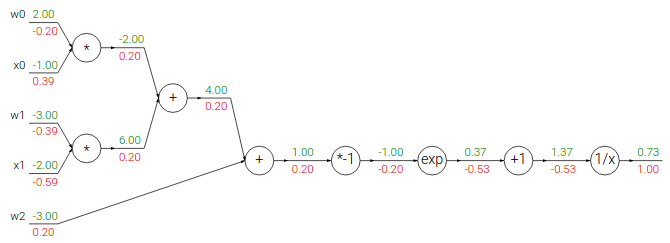
\includegraphics[width=0.7\textwidth]{Images/backprop/3.png}
  \caption{Example circuit for a 2D neuron with a sigmoid activation function. The inputs are $[x0,x1]$ and the (learnable) weights of the neuron are $[w0,w1,w2]$. As we will see later, the neuron computes a dot product with the input and then its activation is softly squashed by the sigmoid function to be in range from 0 to 1.}
\end{figure}

In the example above, we see a long chain of function applications that operates on the result of the dot product between $w,x$. The function that these operations implement is called the sigmoid function $\sigma(x)$. It turns out that the derivative of the sigmoid function with respect to its input simplifies if you perform the derivation (after a fun tricky part where we add and subtract a 1 in the numerator):

\begin{equation}
\sigma(x) = \frac{1}{1+e^{-x}} \\\\
\rightarrow \frac{d\sigma(x)}{dx} = \frac{e^{-x}}{(1+e^{-x})^2} = \left( \frac{1 + e^{-x} - 1}{1 + e^{-x}} \right) \left( \frac{1}{1+e^{-x}} \right) 
= \left( 1 - \sigma(x) \right) \sigma(x)
\end{equation}

As we see, the gradient turns out to simplify and becomes surprisingly simple. For example, the sigmoid expression receives the input 1.0 and computes the output 0.73 during the forward pass. The derivation above shows that the local gradient would simply be (1 - 0.73) * 0.73 ~= 0.2, as the circuit computed before (see the image above), except this way it would be done with a single, simple and efficient expression (and with less numerical issues). Therefore, in any real practical application it would be very useful to group these operations into a single gate. Lets see the backprop for this neuron in code:

\begin{lstlisting}[frame=single]
w = [2,-3,-3] # assume some random weights and data
x = [-1, -2]

# forward pass
dot = w[0]*x[0] + w[1]*x[1] + w[2]
f = 1.0 / (1 + math.exp(-dot)) # sigmoid function

# backward pass through the neuron (backpropagation)
ddot = (1 - f) * f # gradient on dot variable, using the sigmoid gradient derivation
dx = [w[0] * ddot, w[1] * ddot] # backprop into x
dw = [x[0] * ddot, x[1] * ddot, 1.0 * ddot] # backprop into w
# we're done! we have the gradients on the inputs to the circuit
\end{lstlisting}

\paragraph*{Implementation protip} staged backpropagation. As shown in the code above, in practice it is always helpful to break down the forward pass into stages that are easily backpropped through. For example here we created an intermediate variable \texttt{dot} which holds the output of the dot product between \texttt{w} and \texttt{x}. During backward pass we then successively compute (in reverse order) the corresponding variables (e.g. \texttt{ddot}, and ultimately \texttt{dw}, \texttt{dx}) that hold the gradients of those variables.

The point of this section is that the details of how the backpropagation is performed, and which parts of the forward function we think of as gates, is a matter of convenience. It helps to be aware of which parts of the expression have easy local gradients, so that they can be chained together with the least amount of code and effort.


\section*{Backprop in practice: Staged computation}

Lets see this with another example. Suppose that we have a function of the form:
\begin{equation}
f(x,y) = \frac{x + \sigma(y)}{\sigma(x) + (x+y)^2}
\end{equation}
To be clear, this function is completely useless and it’s not clear why you would ever want to compute its gradient, except for the fact that it is a good example of backpropagation in practice. It is very important to stress that if you were to launch into performing the differentiation with respect to either $x$ or $y$, you would end up with very large and complex expressions. However, it turns out that doing so is completely unnecessary because we don’t need to have an explicit function written down that evaluates the gradient. We only have to know how to compute it. Here is how we would structure the forward pass of such expression:

\begin{lstlisting}[frame=single]
x = 3 # example values
y = -4

# forward pass
sigy = 1.0 / (1 + math.exp(-y)) # sigmoid in numerator   #(1)
num = x + sigy # numerator                               #(2)
sigx = 1.0 / (1 + math.exp(-x)) # sigmoid in denominator #(3)
xpy = x + y                                              #(4)
xpysqr = xpy**2                                          #(5)
den = sigx + xpysqr # denominator                        #(6)
invden = 1.0 / den                                       #(7)
f = num * invden # done!                                 #(8)
\end{lstlisting}

Phew, by the end of the expression we have computed the forward pass. Notice that we have structured the code in such way that it contains multiple intermediate variables, each of which are only simple expressions for which we already know the local gradients. Therefore, computing the backprop pass is easy: We’ll go backwards and for every variable along the way in the forward pass (\texttt{sigy, num, sigx, xpy, xpysqr, den, invden}) we will have the same variable, but one that begins with a \texttt{d}, which will hold the gradient of the output of the circuit with respect to that variable. Additionally, note that every single piece in our backprop will involve computing the local gradient of that expression, and chaining it with the gradient on that expression with a multiplication. For each row, we also highlight which part of the forward pass it refers to:

\begin{lstlisting}[frame=single]
# backprop f = num * invden
dnum = invden # gradient on numerator                             #(8)
dinvden = num                                                     #(8)
# backprop invden = 1.0 / den 
dden = (-1.0 / (den**2)) * dinvden                                #(7)
# backprop den = sigx + xpysqr
dsigx = (1) * dden                                                #(6)
dxpysqr = (1) * dden                                              #(6)
# backprop xpysqr = xpy**2
dxpy = (2 * xpy) * dxpysqr                                        #(5)
# backprop xpy = x + y
dx = (1) * dxpy                                                   #(4)
dy = (1) * dxpy                                                   #(4)
# backprop sigx = 1.0 / (1 + math.exp(-x))
dx += ((1 - sigx) * sigx) * dsigx # Notice += !! See notes below  #(3)
# backprop num = x + sigy
dx += (1) * dnum                                                  #(2)
dsigy = (1) * dnum                                                #(2)
# backprop sigy = 1.0 / (1 + math.exp(-y))
dy += ((1 - sigy) * sigy) * dsigy                                 #(1)
# done! phew
\end{lstlisting}

Notice a few things:

\paragraph*{Cache forward pass variables} To compute the backward pass it is very helpful to have some of the variables that were used in the forward pass. In practice you want to structure your code so that you cache these variables, and so that they are available during backpropagation. If this is too difficult, it is possible (but wasteful) to recompute them.

\paragraph*{Gradients add up at forks} The forward expression involves the variables $x,y$ multiple times, so when we perform backpropagation we must be careful to use \texttt{+=} instead of \texttt{=} to accumulate the gradient on these variables (otherwise we would overwrite it). This follows the multivariable chain rule in Calculus, which states that if a variable branches out to different parts of the circuit, then the gradients that flow back to it will add.


\section*{Patterns in backward flow}

It is interesting to note that in many cases the backward-flowing gradient can be interpreted on an intuitive level. For example, the three most commonly used gates in neural networks (add,mul,max), all have very simple interpretations in terms of how they act during backpropagation. Consider this example circuit:

\begin{figure}[h]
  \centering
  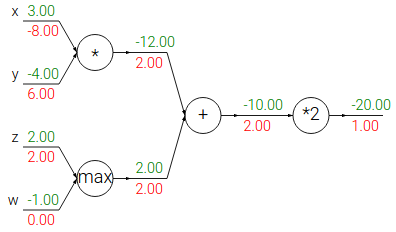
\includegraphics[width=0.4\textwidth]{Images/backprop/4.png}
  \caption{An example circuit demonstrating the intuition behind the operations that backpropagation performs during the backward pass in order to compute the gradients on the inputs. Sum operation distributes gradients equally to all its inputs. Max operation routes the gradient to the higher input. Multiply gate takes the input activations, swaps them and multiplies by its gradient.
}
\end{figure}

Looking at the diagram above as an example, we can see that:

\paragraph*{add gate} The add gate always takes the gradient on its output and distributes it equally to all of its inputs, regardless of what their values were during the forward pass. This follows from the fact that the local gradient for the add operation is simply +1.0, so the gradients on all inputs will exactly equal the gradients on the output because it will be multiplied by x1.0 (and remain unchanged). In the example circuit above, note that the + gate routed the gradient of 2.00 to both of its inputs, equally and unchanged.

\paragraph*{max gate} The max gate routes the gradient. Unlike the add gate which distributed the gradient unchanged to all its inputs, the max gate distributes the gradient (unchanged) to exactly one of its inputs (the input that had the highest value during the forward pass). This is because the local gradient for a max gate is 1.0 for the highest value, and 0.0 for all other values. In the example circuit above, the max operation routed the gradient of 2.00 to the z variable, which had a higher value than w, and the gradient on w remains zero.

\paragraph*{multiply gate} The multiply gate is a little less easy to interpret. Its local gradients are the input values (except switched), and this is multiplied by the gradient on its output during the chain rule. In the example above, the gradient on x is -8.00, which is -4.00 x 2.00.

Unintuitive effects and their consequences. Notice that if one of the inputs to the multiply gate is very small and the other is very big, then the multiply gate will do something slightly unintuitive: it will assign a relatively huge gradient to the small input and a tiny gradient to the large input. Note that in linear classifiers where the weights are dot producted $w^Tx_i$ (multiplied) with the inputs, this implies that the scale of the data has an effect on the magnitude of the gradient for the weights. For example, if you multiplied all input data examples $x_i$ by 1000 during preprocessing, then the gradient on the weights will be 1000 times larger, and you’d have to lower the learning rate by that factor to compensate. This is why preprocessing matters a lot, sometimes in subtle ways! And having intuitive understanding for how the gradients flow can help you debug some of these cases.


\section*{Gradients for vectorized operations}

The above sections were concerned with single variables, but all concepts extend in a straight-forward manner to matrix and vector operations. However, one must pay closer attention to dimensions and transpose operations.

\paragraph*{Matrix-Matrix multiply gradient} Possibly the most tricky operation is the matrix-matrix multiplication (which generalizes all matrix-vector and vector-vector) multiply operations:

\begin{lstlisting}[frame=single]
# forward pass
W = np.random.randn(5, 10)
X = np.random.randn(10, 3)
D = W.dot(X)

# now suppose we had the gradient on D from above in the circuit
dD = np.random.randn(*D.shape) # same shape as D
dW = dD.dot(X.T) #.T gives the transpose of the matrix
dX = W.T.dot(dD)
\end{lstlisting}

\textbf{Tip}: use dimension analysis! Note that you do not need to remember the expressions for \texttt{dW} and \texttt{dX} because they are easy to re-derive based on dimensions. For instance, we know that the gradient on the weights \texttt{dW} must be of the same size as \texttt{W} after it is computed, and that it must depend on matrix multiplication of \texttt{X} and \texttt{dD} (as is the case when both \texttt{X,W} are single numbers and not matrices). There is always exactly one way of achieving this so that the dimensions work out. For example, \texttt{X} is of size [10 x 3] and \texttt{dD} of size [5 x 3], so if we want \texttt{dW} and \texttt{W} has shape [5 x 10], then the only way of achieving this is with \texttt{dD.dot(X.T)}, as shown above.

\paragraph*{Work with small, explicit examples}. Some people may find it difficult at first to derive the gradient updates for some vectorized expressions. Our recommendation is to explicitly write out a minimal vectorized example, derive the gradient on paper and then generalize the pattern to its efficient, vectorized form.

Erik Learned-Miller has also written up a longer related document on taking matrix/vector derivatives which you might find helpful. Find it here.


\section*{Summary}
\begin{itemize}
\item We developed intuition for what the gradients mean, how they flow backwards in the circuit, and how they communicate which part of the circuit should increase or decrease and with what force to make the final output higher.
\item We discussed the importance of staged computation for practical implementations of backpropagation. You always want to break up your function into modules for which you can easily derive local gradients, and then chain them with chain rule. Crucially, you almost never want to write out these expressions on paper and differentiate them symbolically in full, because you never need an explicit mathematical equation for the gradient of the input variables. Hence, decompose your expressions into stages such that you can differentiate every stage independently (the stages will be matrix vector multiplies, or max operations, or sum operations, etc.) and then backprop through the variables one step at a time.
\end{itemize}

In the next section we will start to define Neural Networks, and backpropagation will allow us to efficiently compute the gradients on the connections of the neural network, with respect to a loss function. In other words, we’re now ready to train Neural Nets, and the most conceptually difficult part of this class is behind us! ConvNets will then be a small step away.
\chapter{Parameters Update}

IMPORTANT NOTATION!!: Through all this chapter I am saying parameters = weights, but remember that there are other ones like the bias.

\section*{First Order Optimization Methods}
The pseudo-code for updating the parameters:
\begin{lstlisting}[frame=single]
while True:
     data_batch = dataset.sample_data_batch()
     loss = network.forward(data_batch)
     dw = network.backward()
     w += -learning_rate * dw
\end{lstlisting}

This update (\texttt{w+=-lr*dw}) is an stochastic gradient descent. Let's see better ways of updating the parameters. The plot below shows different update strategies to optimize the loss function. In DNN, as you scale your model, local minima become less and less of an issue. The loss function shape we should have in mind is like a landskape with a lot of local minima but all with more or less the same loss. As you scale the model the distance between the bigger and lower local minima scales down (there is no bad local minima in big networks).

\subsection*{Stochastic gradient descent}
\begin{equation}
w_t = w_{t-1} -\alpha \bigtriangleup L(w_{t-1})
\end{equation}

where $\bigtriangleup L(w_{t-1})$ is the derivative of the loss function and  the learning rate

\begin{figure}[h]
  \centering
  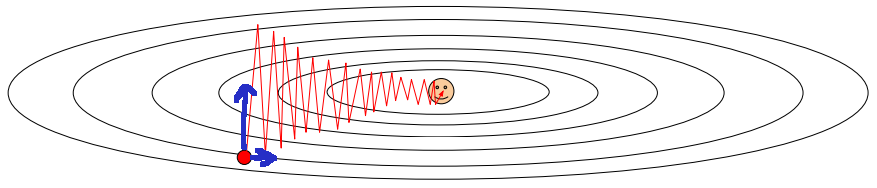
\includegraphics[width=0.6\textwidth]{Images/params_up/1.png}
  \caption{SGD example}
\end{figure}

\textbf{Problem:}
Supose a 2dimensions loss function (NN with 2 layers and 2 weights) which is steep vertically and shallow horizontally (weight represented in the vertical axis has a higher impact over the loss function). The horizontal gradient is small because it is a shallow function in the horizontal direction, and a big gradient in the vertical direction because it is steep in this direction. Then, the update is way too slow in the horizontal direction, and to fast in the vertical direction. This causes an ugly jerk shape.

Notice that it is not an option to just decrease the learning rate because then it would take forever to cross all the shallow surface.

IMPORTANT NOTATION!!: Through all this chapter I am saying parameters = weights, but remember that there are other ones like the bias.

\subsection*{Momentum update}
\begin{equation}
\begin{aligned}
v_0 &= 0 \\
v_t &= \mu v_{t-1} - \alpha \bigtriangleup L(w_{t-1}) \\
w_t &= w_{t-1} + v_t
\end{aligned}
\end{equation}

where $\mu \in [0,1]$ and usually takes values around ~0.5, ~0.9 or 0.99 (sometimes annealed over time 0.5 -> 0.99)

It can be interpreted as a ball rolling across the loss function starting at velocity 0. Notice that  would represent position,  velocity,  friction (decreasing velocity over time). Now you will speed up in shallow surfaces directions and in steep directions you will be jiggly but you will have a force pushing you to the center (like a ball rolling in a convex function).


In the first plot we can see that first it overshoots because of all the accumulated velocity but it ends converging to the minimum quicker than SVG.

\subsection*{Nesterov Momentum update (or Nesterov accelerated gradient descent) }
\begin{equation}
\begin{aligned}
v_0 &= 0 \\
v_t &= \mu v_{t-1} - \alpha \bigtriangleup L(w_{t-1} + \mu v_{t-1}) \\
w_t &= w_{t-1} + v_t
\end{aligned}
\end{equation}
A slightly different version of the momentum update has recently been gaining popularity. It enjoys stronger theoretical converge guarantees for convex functions and in practice it also consistenly works slightly better than standard momentum.

The core idea behind Nesterov momentum is that when the current parameter vector is at some position $x$ (weights), then looking at the momentum update above, we know that the momentum term alone (i.e. ignoring the second term with the gradient) is about to nudge the parameter vector by $\mu * v$. Therefore, if we are about to compute the gradient, we can treat the future approximate position $x + \mu * v$ as a “lookahead” - this is a point in the vicinity of where we are soon going to end up. Hence, it makes sense to compute the gradient at $x + \mu * v$ instead of at the “old/stale” position $x$.

\begin{figure}[h]
  \centering
  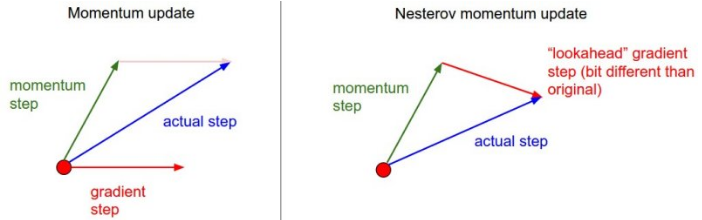
\includegraphics[width=0.7\textwidth]{Images/params_up/2.png}
  \caption{Nesterov Momentum update}
\end{figure}

IMPORTANT NOTATION!!: Through all this chapter I am saying parameters = weights, but remember that there are other ones like the bias.

\subsection*{AdaGrad} 
\begin{equation}
\begin{aligned}
c_t &= c_{t-1} + \bigtriangleup L(w_{t-1})^2 \\
w_t &= w_{t-1} - \frac{\alpha  \bigtriangleup L(w_{t-1})}{\sqrt{c_t} + 1^{-7}}
\end{aligned}
\end{equation}

where  is the cache is a giant vector of the same size of your parameter vector . So this cache keeps track of the sum of squares (or also called the uncentered second moment) of your parameters in each direction (array). So now, with the cache, each dimension of the parameter vector has a different dynamic learning rate which is dynamically scaled based on what kind of gradients are you seeing in terms of their scale.

In the first case explained steep vertically and shallow horizontally loss function (2 weights). We have a large gradient vertically which will be added to cache. So in the vertical direction, the parameter update will be getting smaller and smaller (= smaller steps) because the denominator keeps increasing (= learning rate keeps decreasing). In the horizontal direction the surface is shallow, so  will be small and as a consequence the learning rate will not decrease.  The horizontal direction will have faster progress relative to the vertical direction.

So the cache is acting as an equalizer accounting for the stiffness ( ) of the loss function in the parameters direction. Keep in mind that this equalizer effect over a specific parameter (=weight) is independent of the rest of parameters. It is not like a normalization.

Problem: When training over long time the step size (= learning rate) goes to 0 and the network stops learning. To solve this, the next method is proposed.

\subsection*{RMSProp}
\begin{equation}
\begin{aligned}
c_t &= \gamma c_{t-1} + (1-\gamma) \bigtriangleup L(w_{t-1})^2 \\
w_t &= w_{t-1} - \frac{\alpha  \bigtriangleup L(w_{t-1})}{\sqrt{c} + 1^{-7}}
\end{aligned}
\end{equation}
The idea is that instead of keeping the sum of squares in every direction of the parameters, we make the counter leaky by introducing the decay rate . So we maintain the nice effect of equalizing the directions but it will not converge to 0. The term  is there just to prevent the division by 0.

You can also imagine the decay rate as a sort of a forgetting factor that makes the cache  only a function of the last few gradient but in an exponential weighted sum rate. Also, notice that we could not do something like having a sliding window just to track the previous n gradients because it would take too much memory.

Comparing RMSProp vs AdaGrad in DNNs, in practice AdaGrad usually ends up stopping too early.

IMPORTANT NOTATION!!: Through all this chapter I am saying parameters = weights, but remember that there are other ones like the bias.

\subsection*{Adam update - USE THIS ONE}
\begin{equation}
\begin{aligned}
v_0 = c_0 = 0
v_t = \frac{\mu v_{t-1} + (1-\mu)\bigtriangleup L (w_{t-1})}{1 - \mu^t} \\
c_t = \frac{\gamma c_{t-1} + (1-\gamma)\bigtriangleup L (w_{t-1})^2}{1 - \gamma^t} \\
w_t &= w_{t-1} - \frac{\alpha v_t}{\sqrt{c} + 1^{-7}}
\end{aligned}
\end{equation}
Adam update is a combination of adaptive scaling (AdaGrad) and momentum (Momentum update).  is the velocity and  the cache. Sometimes  and   are detonated first and second momentum, respectively. To compensate the fact that the momentums are initialized to zero () and need some time to "warm up", we introduce a bias correction in order to scale up  and  in the first iterations so you do not get a very biased estimate of the first and second momentum.
bias correction: $ \frac{1}{1 - \mu^t}, \frac{1}{1 - \gamma^t},$


So in DNNs you are in a stochastic setting, you are sampling from a mini-batch, there is going to be a lot of randomness in the forward pass. In other words, you are getting a lot of noisy gradients.

\begin{itemize}
\item Momentum contribution: So instead of using every gradient at every single time step we only use the decaying sum of previous gradients which helps use stabilize your gradient direction a bit.
\item Cache contribution: To make sure that  the steps size workout in steep and shallow directions.
\end{itemize}

Usually $\mu = 0.9, \gamma = 0.995$ but if you cross-validate them it can help a bit.

Why using momentum update instead of Nesterov Momentum update? It could be also done but it does not make such a difference.

IMPORTANT NOTATION!!: Through all this chapter I am saying parameters = weights, but remember that there are other ones like the bias.


\subsection*{Learning Rate - Decay over time}

So which is the best learning rate for training DNNs?
None. The best one is to start with high learning first because it optimizes faster than the "good learning rate", in this way you do really fast progress. But at some point you are going to be too stochastic and you can not converge to a minimum. So, at this point you must start decreasing the learning rate.

\begin{figure}[h]
  \centering
  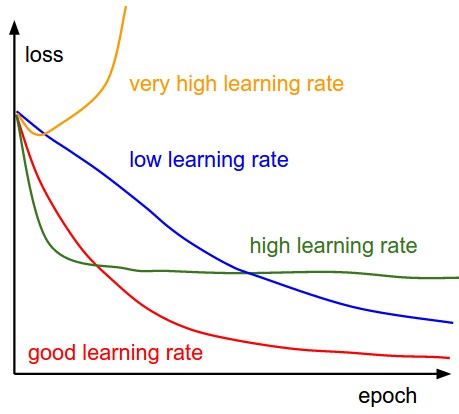
\includegraphics[width=0.35\textwidth]{Images/params_up/3.jpeg}
  \caption{Learning rate selection}
\end{figure}

Another way of seeing it is to have in mind is that with a high learning rate, the system contains too much kinetic energy and the parameter vector bounces around chaotically, unable to settle down into deeper, but narrower parts of the loss function.

 Knowing when to decay the learning rate can be tricky: Decay it slowly and you’ll be wasting computation bouncing around chaotically with little improvement for a long time. But decay it too aggressively and the system will cool too quickly, unable to reach the best position it can. There are three common types of implementing the learning rate decay:

\begin{itemize}
\item \textbf{Step decay}: Reduce the learning rate by some factor every few epochs. Typical values might be reducing the learning rate by a half every 5 epochs, or by 0.1 every 20 epochs. These numbers depend heavily on the type of problem and the model. One heuristic you may see in practice is to watch the validation error while training with a fixed learning rate, and reduce the learning rate by a constant (e.g. 0.5) whenever the validation error stops improving.
\item \textbf{Exponential decay} has the mathematical form $\alpha = \alpha_0 e^{-kt}$, where $\alpha_0, k$ are hyperparameters and  is the iteration number (but you can also use units of epochs).
\item \textbf{1/t decay} has the mathematical form $\alpha = \frac{\alpha_0}{1+Kt}$ where $\alpha_0, k$ are hyperparameters and is the iteration number.
\end{itemize}


In practice, we find that the step decay dropout is slightly preferable because the hyperparameters it involves (the fraction of decay and the step timings in units of epochs) are more interpretable than the hyperparameter $k$. Lastly, if you can afford the computational budget, err on the side of slower decay and train for a longer time.

Notice that Adagrad, RMSProp and Adam already have a learning decay. When using this methods it may help a little bit also adding a learning decay method. For SGD and SGD+Momentum you should always add the learning decay.

\section*{Second Order Optimization Methods}
The advantages of second order optimization methods are: faster convergence and no hyper-parameters. However they are not normally used because they are to heavy, to much staff happening, and they use too much memory. It is preferable just to use first order methods.

The idea of second order methods is that they approximate the loss function in a more precise way. As first order methods, they approximate with an hyperplane of like which way are we sloping. Also they also approximate with Hessian (H) which is telling you how is this surface curving. So you need the gradient for the sloping estimation and the Hessian for the surface curvature.

For example in the Newton method, ones you have form this bowl like Hessian approximation to you objective function, you can use this information to jump directly to the minimum of that approximation, and you keep iterating this strategy.

\begin{equation}
\begin{aligned}
J(\theta) &\approx J(\theta_0) + (\theta - \theta_0)^T \bigtriangleup_{\theta}J(\theta_0) + \frac{1}{2}(\theta - \theta_0)^T H (\theta - \theta_0)
\theta^\ast &= \theta_0 - H^{-1}\bigtriangleup_{\theta}J(\theta_0)
\end{aligned}
\end{equation}

This method is impractical to train DNNs because it would take too much memory. So imagine you have 10 million parameters, then your Hessian matrix would of size 10 million by 10 million and then you want to invert it, so good luck.

There is a variant of the Newton method called BGFS which approximates the inverse Hessian with rank 1 over time so you do not need to compute the inverse of the Hessian but still requires to store the gigantic matrix in memory.

Another extension called L-BGFS does not require you to store all the full inverse matrix. This method is used some time to train DNNs. It usually works very good in full batch and deterministic functions with no stochastic settings. However, it does not transfer very well to mini-batch settings because the approximation it is doing of the Hessian matrix are incorrect when you switch the batch. Also, it does not work well with stochastic settings, so you have to remove all sources of randomness (e.g. dropout). Still, it is to heavy, to much staff is happening,f and it is better just to use first order methods.

\section*{Summary}
\begin{itemize}
\item Adam is a good default choice in most cases. Some times it helps adding learning rate decay like step decay or exponential decay even-though Adam already has inside a learning decay.
\item If you can afford to do full batch updates then try out L-BFGS (do not forget to disable all sources of noise/randomness)
\item Decay your learning rate over the period of the training. For example, halve the learning rate after a fixed number of epochs, or whenever the validation accuracy tops off.
\end{itemize}

IMPORTANT NOTATION!!: Through all this chapter I am saying parameters = weights, but remember that there are other ones like the bias.
\chapter{Dropout}
\begin{figure}[!htb]
  \centering
  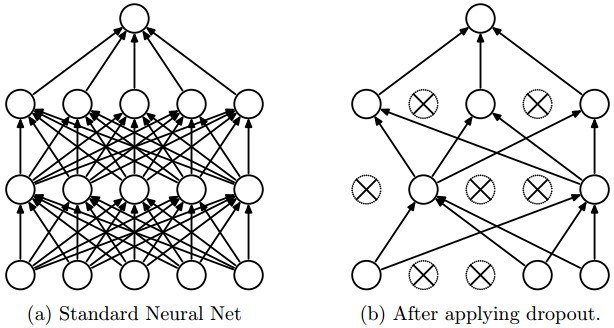
\includegraphics[width=0.5\textwidth]{Images/dropout/1.jpeg}
  \caption{Dropout}
\end{figure}
``Randomly set ~\%50 some neurons to zero in the forward pass."  There two ways of understanding why this works:
\begin{itemize}
\item This makes the network unable to relay on a single feature. Thus, forcing it to generate redundant representation. In this way, you will be representing an object with redundant descriptors, detectors, etc. So in test time, if some features can not be detected, you still can really on the other ones.

\begin{figure}[!htb]
  \centering
  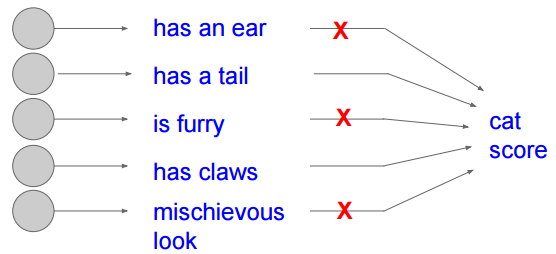
\includegraphics[width=0.45\textwidth]{Images/dropout/3.png}
  \caption{Relay on multiple features}
\end{figure}

\item It can also be seen as training a large ensemble of models that share parameters. When applying a mask to shutdown some randomly neurons at the forward pass this mask stays there for the backward pass. Thus, in the backprop step, no gradient will flow through the neurons that were shut off to zero; so its weights to the previous layer will not be updated. In other words, the neurons that were dropout do not update their connections to the previous layer, just as if they were not there. With dropout you are subsampeling a part of your neural network and training it with the current example. So each binary mask is one model which gets trained on only ~one datapoint (or more in the case that two random mask are equal during training).
\end{itemize}

\textbf{WARNING}: If dropout is not working for you, you should probably be using a bigger network.

\subsection*{Train time}
During the forward pass set ~50\% of the neurons to 0. To get an idea the code below shows a naive implementation of dropout 
\begin{lstlisting}[frame=single] 
""" Vanilla Dropout: Not recommended implementation (see notes below) """

p = 0.5 # probability of keeping a unit active. higher = less dropout

def train_step(X):
  """ X contains the data """

  # forward pass for example 3-layer neural network
  H1 = np.maximum(0, np.dot(W1, X) + b1)
  U1 = np.random.rand(*H1.shape) < p # first dropout mask
  H1 *= U1 # drop!
  H2 = np.maximum(0, np.dot(W2, H1) + b2)
  U2 = np.random.rand(*H2.shape) < p # second dropout mask
  H2 *= U2 # drop!
  out = np.dot(W3, H2) + b3

  # backward pass: compute gradients... (not shown)
  # perform parameter update... (not shown)
 \end{lstlisting}

\subsection*{Test time}
At test time ideally we would like to integrate out all the noise (not possible). A Monte Carlo approximation would be: do many forward passes with different dropout masks, average all predictions. Unfortunately its not time efficient. Instead, you can approximate this method without not droping out any unit in the forward pass during testing but we have to be careful. 

\subsubsection*{Example}
\begin{figure}[!htb]
  \centering
  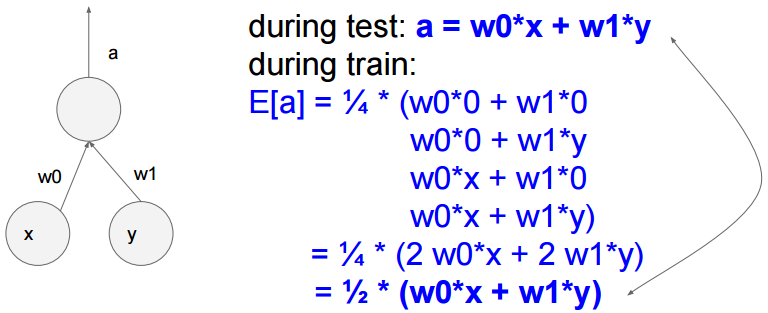
\includegraphics[width=0.45\textwidth]{Images/dropout/2.png}
  \caption{Example}
\end{figure}
Imagine this linear NN and a dropout $prob = 0.5$. During training time the expected value is the average between all the possible masks activation value. However, if we use all the neurons in test time, the activation value is going to be twice the expected value in train time. So it is easy to see that this half comes from the fact that at train time we dropout neurons with probability 50\%.

With $p=0.5$ dropout prob, using all inputs in the forward pass would inflate the activations by $2x$ from what the network was "used to" during training. Thus, you have to compensate by scaling the activations back down by $1/2$. In this way, the ouput at test time is equal to the expected output at training time. Let's see a naive implementation:
\begin{lstlisting}[frame=single] 
""" Vanilla Dropout: Not recommended implementation (see notes below) """

p = 0.5 # probability of keeping a unit active. higher = less dropout

def predict(X):
  # ensembled forward pass
  H1 = np.maximum(0, np.dot(W1, X) + b1) * p # NOTE: scale the activations
  H2 = np.maximum(0, np.dot(W2, H1) + b2) * p # NOTE: scale the activations
  out = np.dot(W3, H2) + b3
\end{lstlisting}

A better way of implementing dropout is using "inverted dropout". The idea is very simple, instead of multiplying the activation values by the dropout probability during test time, divide the training activation values by the dropout probability during train time.  In this way, test time is unchanged.

\begin{lstlisting}[frame=single]
"""
Inverted Dropout: Recommended implementation example.
We drop and scale at train time and don't do anything at test time.
"""

p = 0.5 # probability of keeping a unit active. higher = less dropout

def train_step(X):
  # forward pass for example 3-layer neural network
  H1 = np.maximum(0, np.dot(W1, X) + b1)
  U1 = (np.random.rand(*H1.shape) < p) / p # first dropout mask. Notice /p!
  H1 *= U1 # drop!
  H2 = np.maximum(0, np.dot(W2, H1) + b2)
  U2 = (np.random.rand(*H2.shape) < p) / p # second dropout mask. Notice /p!
  H2 *= U2 # drop!
  out = np.dot(W3, H2) + b3

  # backward pass: compute gradients... (not shown)
  # perform parameter update... (not shown)

def predict(X):
  # ensembled forward pass
  H1 = np.maximum(0, np.dot(W1, X) + b1) # no scaling necessary
  H2 = np.maximum(0, np.dot(W2, H1) + b2)
  out = np.dot(W3, H2) + b3
\end{lstlisting}

There is a method to dropout single weights instead of full neurons call dropconnect
\chapter{Hyper-Parameters selection and babysitting}

\section*{Sanity test}
Make sure that you can overfit very small portion of the training data. Take ~20 samples, turn off regularization and make sure that you can get a loss of ~0. If you can't overfit there is a problem: or there is something broken or you have to scale up your network.

\section*{Learning Rate}
Start with small regularization (0.00001) and find learning rate that makes the loss not go down.  Then, find learning rate that makes the loss go down but at some point it explodes. The learning rate is in between this range.
\begin{figure}[h]
  \centering
  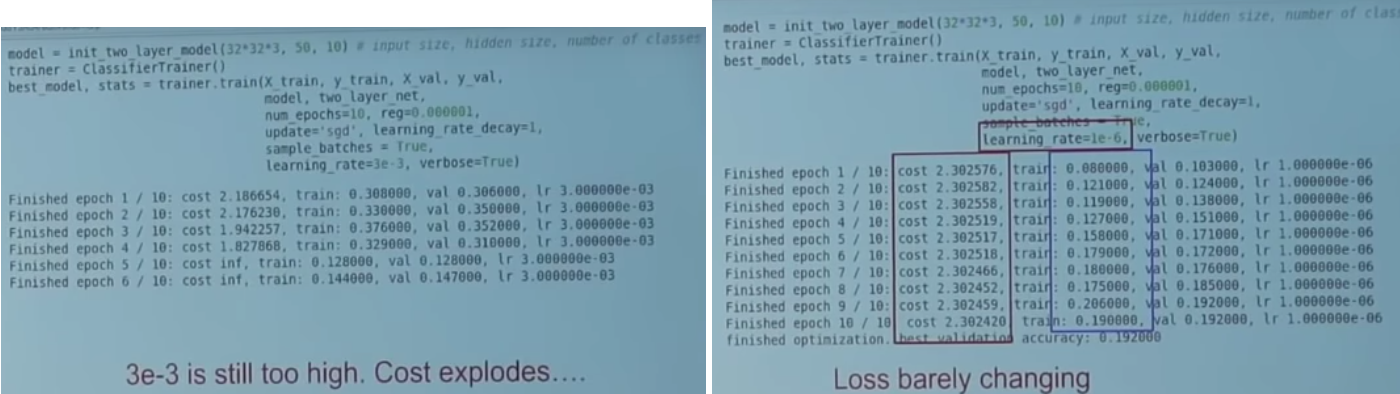
\includegraphics[width=\textwidth]{Images/hyper_params_tun/9.png}
  \caption{\textbf{Left}: Loss exploding, \textbf{Right}: Loss not going down}
\end{figure}
\begin{itemize}
\item Loss not going down: learning rate too low. Something funny can happen in this case. Loss not going down but accuracy improving until ~20\%. How is that possible? So because of the way softmax is computed, small changes in the lost can cause small changes in the scores which make the correct class has a tiny bigger score than the others. This, makes the softmax classifier get more samples correct.
\item Loss exploding (NaN happens): learning rate too high
\end{itemize}



\section*{Hyperparameter Optimization - Coarse to fine serach}
Tuning regularization and learning rate. Do coarse -> fine for cross-validation in stages. In other words, first do a rough search, see what it works, and keep iterating to longer narrow in ranges that are working. First, only a few epochs to get rough idea of what parameters work (few minutes is enough). Second, longer running time, finer search.

Also, it is better to optimize parameters in log space because reg and learning rate work manipulatively in the dynamics of your back propagation.

\begin{figure}[h]
  \centering
  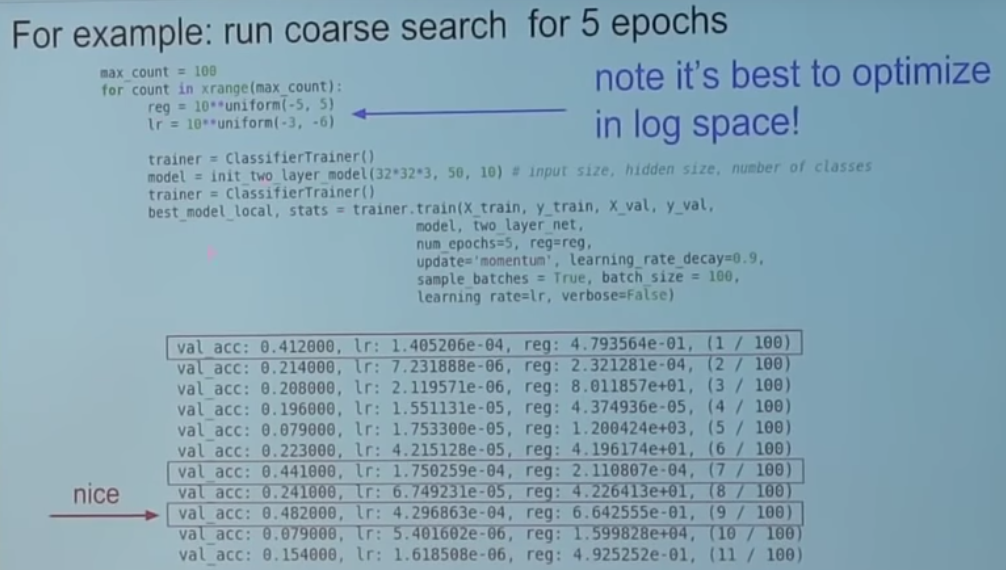
\includegraphics[width=0.6\textwidth]{Images/hyper_params_tun/3.png}
  \caption{First pass - coarse search}
\end{figure}

\begin{figure}[h]
  \centering
  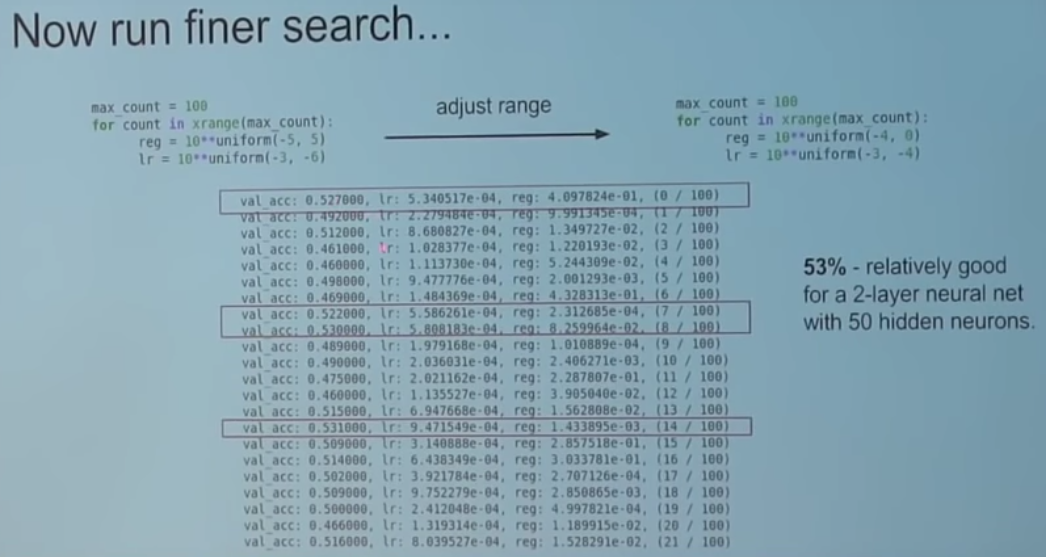
\includegraphics[width=0.6\textwidth]{Images/hyper_params_tun/4.png}
  \caption{Second pass - finer search. Notice that there is a problem with this result. The best result (last red box) has a lr close to the boundary of search that we have set (-3). So it may we better results waiting for lower values of lr. \textbf{Careful with best values on border}}
\end{figure}


\section*{Hyper-parameter Optimization - NEVER do grid (iterative) search of parameters, do random search}

\begin{figure}[h]
  \centering
  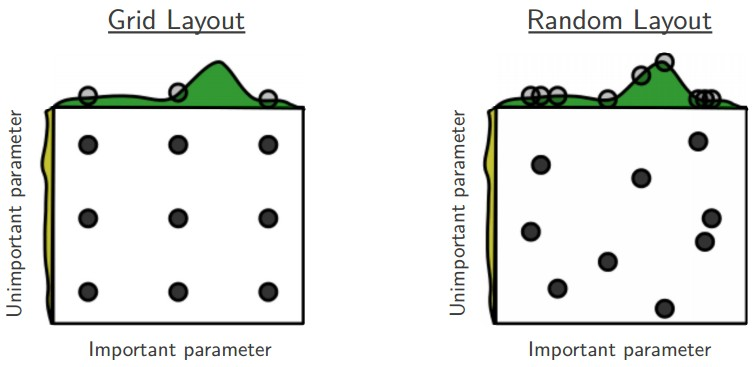
\includegraphics[width=0.5\textwidth]{Images/hyper_params_tun/5.jpeg}
  \caption{Second pass - finer search. Notice that there is a problem with this result. The best result (last red box) has a lr close to the boundary of search that we have set (-3). So it may we better results waiting for lower values of lr. \textbf{Careful with best values on border}}
\end{figure}

For cross-validation, use random search in stead of grid search. The issue is that one of the parameters may be much important than another one.

In this figure in particular its more important the x than the y dimension. Then, with random sampling, your are going to evaluate more different samples of the x parameter space (9 with random vs 3 with grid).

\section*{Hyper-parameter Optimization - Monitor and visualize the loss curve}
\begin{figure}[h]
  \centering
  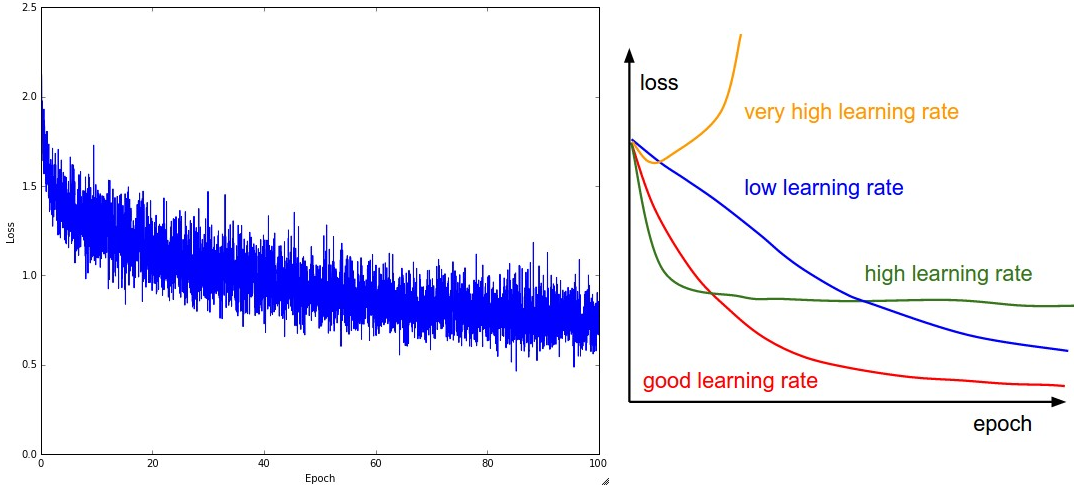
\includegraphics[width=0.65\textwidth]{Images/hyper_params_tun/10.png}
  \caption{In this left case the loss is too slow... The learning rate is too low}
\end{figure}


\section*{Hyper-parameter Optimization - Monitor and visualize the accuracy}
\begin{figure}[h]
  \centering
  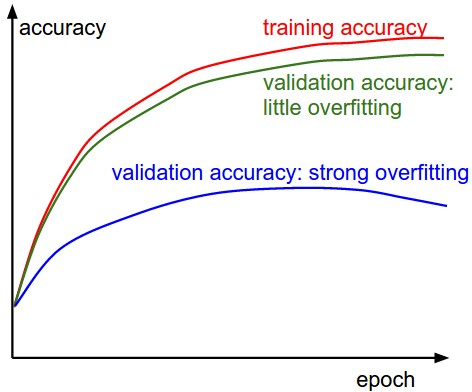
\includegraphics[width=0.3\textwidth]{Images/hyper_params_tun/8.jpeg}
  \caption{Monitor and visualize the accuracy}
\end{figure}
The gap between the training and validation accuracy indicates the amount of overfitting. Two possible cases are shown in the diagram on the left. The blue validation error curve shows very small validation accuracy compared to the training accuracy, indicating strong overfitting (note, it's possible for the validation accuracy to even start to go down after some point). When you see this in practice you probably want to increase regularization (stronger L2 weight penalty, more dropout, etc.) or collect more data. The other possible case is when the validation accuracy tracks the training accuracy fairly well. This case indicates that your model capacity is not high enough: make the model larger by increasing the number of parameters.

\begin{itemize}
\item gap between train\/val is too big: overfitting, increase regularization
\item gap between train\/val too small: increase model capacity
\end{itemize}

In this figure case there is a big gap so it is probably over-fitting. We should increase the regularization factor.

\section*{Hyper-parameter Optimization - Track the ratio of weight updates / weight magnitudes}
You want \texttt{weight\_updates / weight\_magnitudes =~0.001}.
\begin{itemize}
\item If this is too high to decrease learning rate
\item If it is too low to increase learning rate
\end{itemize}


\section*{Dropout not working}
If dropout is not working for you, you should probably be using a bigger network.
\chapter{Other definitions}

\section{Embedding}
An embedding maps an input representation, such as a word or sentence, into a vector. A popular type of embedding are word embeddings such as word2vec or GloVe. We can also embed sentences, paragraphs or images. For example, by mapping images and their textual descriptions into a common embedding space and minimizing the distance between them, we can match labels with images. Embeddings can be learned explicitly, such as in word2vec, or as part of a supervised task, such as Sentiment Analysis. Often, the input layer of a network is initialized with pre-trained embeddings, which are then fine-tuned to the task at hand.

\section{Gradient Clipping}
Gradient Clipping is a technique to prevent exploding gradients in very deep networks, typically Recurrent Neural Networks. There exist various ways to perform gradient clipping, but the a common one is to normalize the gradients of a parameter vector when its L2 norm exceeds a certain threshold according to \texttt{new\_gradients = gradients * threshold / l2\_norm(gradients)}.

\section{Vanishing Gradient Problem}

The vanishing gradient problem arises in very deep Neural Networks, typically Recurrent Neural Networks, that use activation functions whose gradients tend to be small (in the range of 0 from 1). Because these small gradients are multiplied during backpropagation, they tend to “vanish” throughout the layers, preventing the network from learning long-range dependencies. Common ways to counter this problem is to use activation functions like ReLUs that do not suffer from small gradients, or use architectures like LSTMs that explicitly combat vanishing gradients. The opposite of this problem is called the exploding gradient problem.
\chapter{Tricks}


\section*{Real Ensambles}
\begin{itemize}
\item Train multiple independent models
\item At test time average their results
\end{itemize}

Enjoy $\sim 2$\% extra performance.

\section*{Simulated Ensambles}
Fake ensambles. As you are training, normally, you save a checkpoint after each epoch to figure out what was your validation performance at that point. At test time average multiple model checkpoints of a single model.
Enjoy $\sim 1$\% extra performance

\section*{Average parameter vector}
Keep track of (and use at test time) a running average parameter vector. \texttt{params\_test} is a running sum exponentially decaying. One way to visualize it is the following. Think in a case of optimizing a bowl like function and you are bouncing around the minimum, then taking the average of all this steps gets you closer to the minimum.

\begin{lstlisting}[frame=single]
while True:
     data_batch = dataset.sample_data_batch()
     loss = network.forward(data_batch)
     dparams = network.backward()
     params += update_params() //instead of using this parameters at test time
     params_test = 0.995*params_test + 0.005*params //use this ones
\end{lstlisting}

This can give you a small boost.

\section*{Use float32 instead of float64}

Just that. In fact if you can work with float16 do it.

\section*{ReLU bias initialization}
It is a good practice to initialize them with a slightly positive initial bias to avoid "dead neurons".


\chapter{Visualization}

\section{t-SNE visualization}
Embed high-dimensional points so that locally, pairwise distances are conserved i.e. similar things end up in similar places.
Dissimilar things end up wherever. Pronounced "tisni".

\begin{figure}[h]
  \centering
  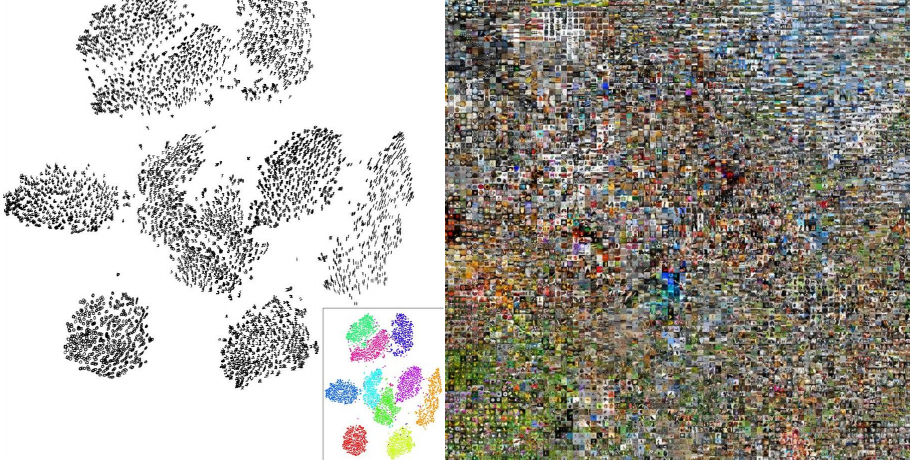
\includegraphics[width=0.6\textwidth]{Images/visualization/16.png}
  \caption{\textbf{Left}: Example embedding of MNIST digits (0-9) in 2D, \textbf{Right}: CIFAR-10 representation warped in a square shape}
\end{figure}

More CIFAR-10 examples \href{http://cs.stanford.edu/people/karpathy/cnnembed/}{here}

\section{Occlusions}
The idea is to create a hit map of the output probability of the CNN of the image in the left corresponding to the correct label as you slide an occlusion across the image.

This helps you understand what are the regions which contains the most valuable features, for the CNN, in the image.

For example, in the first row, we can observe that the probability of the left image being a Pomeranian decreases when we cover its face.

\begin{figure}[h]
  \centering
  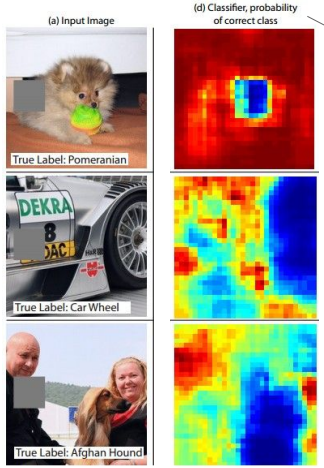
\includegraphics[width=0.25\textwidth]{Images/visualization/3.png}
  \caption{Visualize with occlusions}
\end{figure}


\section{Visualizing Activations}
How can we compute the gradient of any arbitrary neuron in the network w.r.t. the image?

\begin{figure}[h]
  \centering
  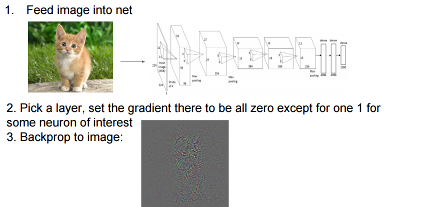
\includegraphics[width=0.6\textwidth]{Images/visualization/4.png}
  \caption{Visualize with occlusions}
\end{figure}

The output image gradients is not that good to understand what is going on. We will now see two strategies to obtain "better looking" gradients: Deconv approaches and

\section{Deconv approaches}

We are trying to see what parts of the input image are exciting a specific neuron. The idea to get a better looking gradient image is only to take into account the positive gradients. In this way we remove the noise caused by mixing positive and negative gradients.

The ReLU layer only backprop the gradient of the activations that where positive at the forward pass.

With Deconv, we must hack this behavior and change it so the ReLU layers only backprop positive gradients and do not care if the forward activations where positive or negative.

\begin{figure}[h]
  \centering
  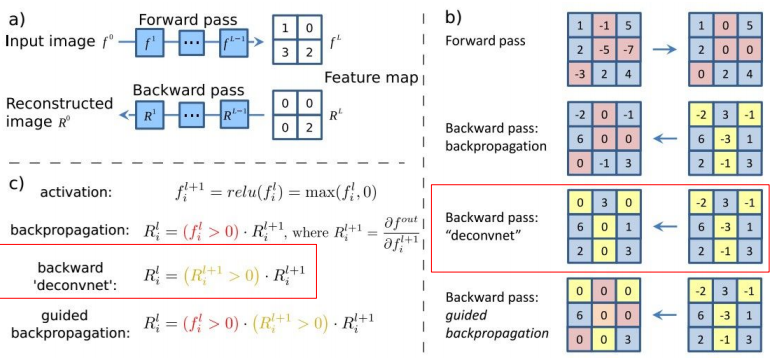
\includegraphics[width=0.8\textwidth]{Images/visualization/5.png}
  \caption{Deconv approaches}
\end{figure}

Now we can show what excites a specific neuron. The figures below show a grid of neurons at each layer. For each neuron we can see the image that arrived to that neuron and what parts of this image excited the neuron. So the deeper the neuron the bigger the area of the original image it observes. Also, it can be seen that the deeper the neuron the higher feature representation.

\begin{figure}[h]
  \centering
  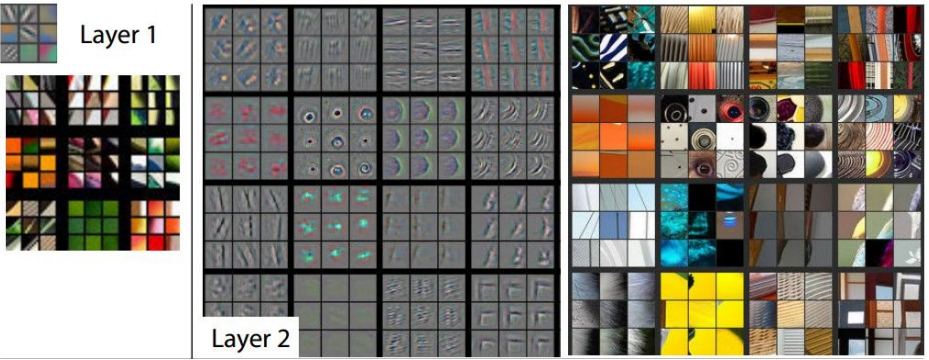
\includegraphics[width=0.8\textwidth]{Images/visualization/6.png}
  \caption{Deconv approaches layers 1 and 2}
\end{figure}

\begin{figure}[h]
  \centering
  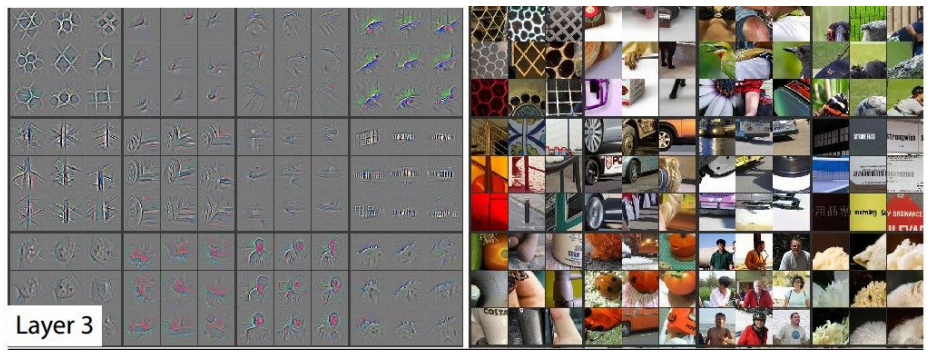
\includegraphics[width=0.8\textwidth]{Images/visualization/7.png}
  \caption{Deconv approaches layer 3}
\end{figure}

\begin{figure}[h]
  \centering
  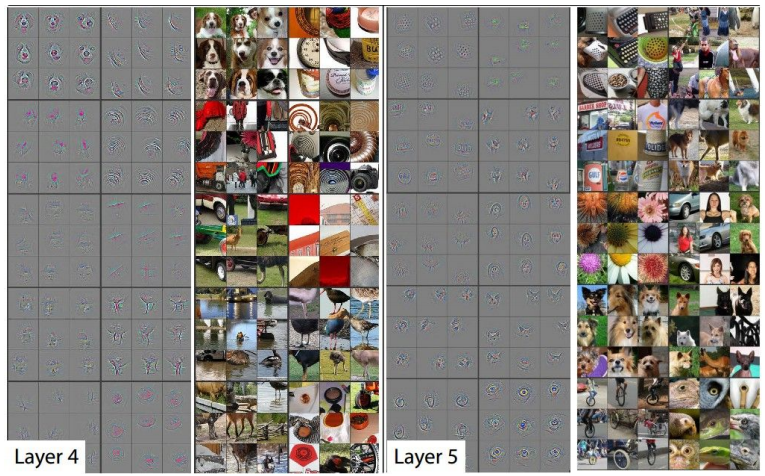
\includegraphics[width=0.8\textwidth]{Images/visualization/8.png}
  \caption{Deconv approaches layers 4 and 5}
\end{figure}


\section{Optimization to image}
How can we find an image that maximizes some class score?
\begin{figure}[h]
  \centering
  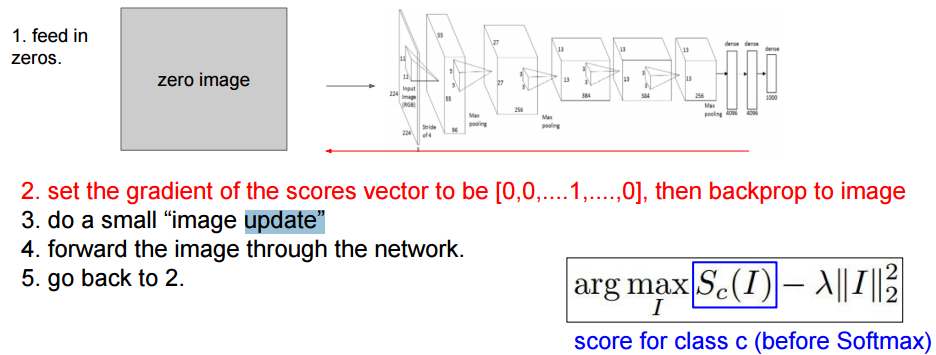
\includegraphics[width=0.6\textwidth]{Images/visualization/9.png}
  \caption{Optimize an image to maximize the score of a specific class}
\end{figure}

\begin{figure}[h]
  \centering
  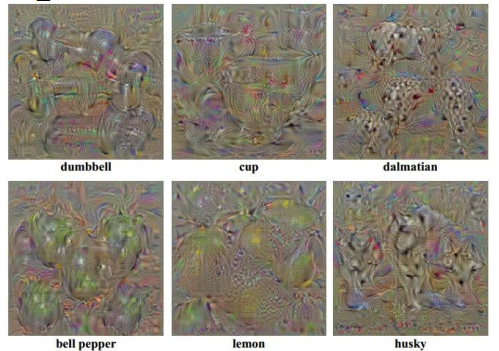
\includegraphics[width=0.45\textwidth]{Images/visualization/10.png}
  \caption{Optimize an image to maximize the score of a specific class output}
\end{figure}


\section{Visualizing Data Gradients}
\begin{enumerate}
\item Feed an input image
\item Set the gradient of the scores vector be [0,0,..,0,1,0,...0] where 1 is the ground-truth label class of the image
\item Backprop to the image
\item For each pixel of the image store the max gradient value across all the channels
\item Plot the gradients
\end{enumerate}

\begin{figure}[h]
  \centering
  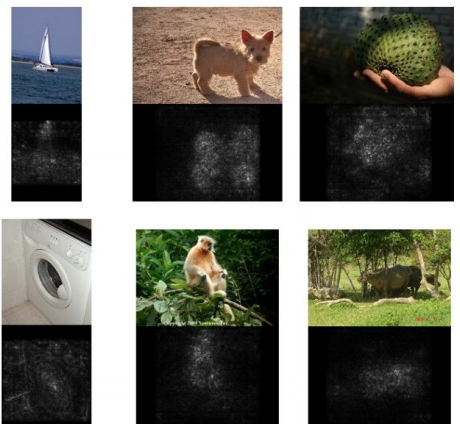
\includegraphics[width=0.3\textwidth]{Images/visualization/11.png}
  \caption{Data gradients output}
\end{figure}


The interpretation of the results are that the staff that is black is not influencing the score of the image. So you can wiggle them and the score will not change. So at the end it is telling you the are of the image that is influencing the network.

\section{DeepDream}

\begin{figure}[h]
  \centering
  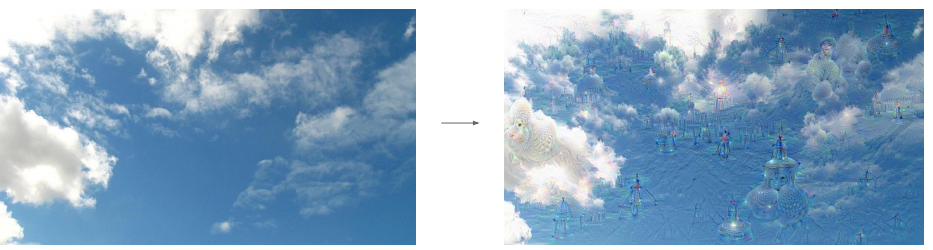
\includegraphics[width=0.6\textwidth]{Images/visualization/13.png}
  \caption{DeepDream output}
\end{figure}

DeepDream \href{http://cs.stanford.edu/people/karpathy/cnnembed/}{link} 

It normally hallucinate a lot of dogs because there are a lot of dog samples in ImageNet (because there are a lot of different dog classes).

\begin{figure}[h]
  \centering
  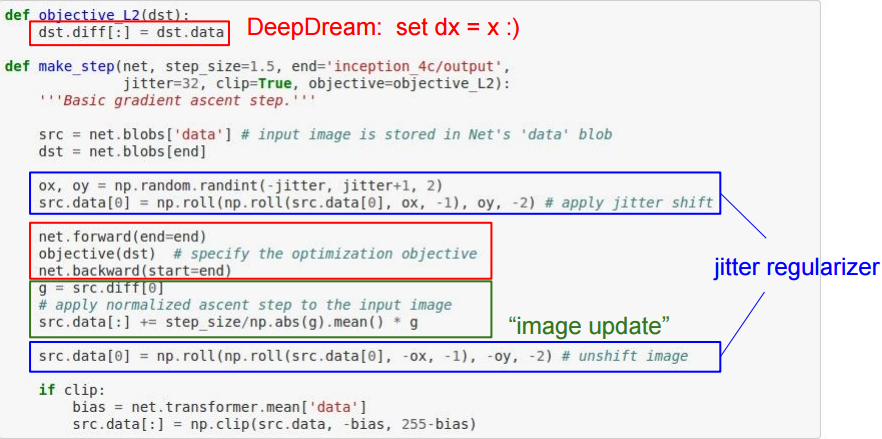
\includegraphics[width=0.8\textwidth]{Images/visualization/12.png}
  \caption{DeepDream code}
\end{figure}

At the end, the only thing DeepDream is doing is: given a layer immediately after a ReLU layer, it sets the gradients equal to the activation values. So if you iteratively update the image with the gradients, you are modifying the image to increase whatever it is exiting the selected layer.

In other words, DeepDream modifies the image in a way that ``boosts” all activations. This creates a feedback loop: e.g. any slightly detected dog face will be made more and more dog like over time.

\section{DeepArt}
Explained at cs231n lecture 9

\section{Adversarial data - Fooling networks}
It is very simple to fool a CNN. Images are super high dimensional objects (one dimension for each pixel). The training images are constrained to a small manifold and we are training ConvNets over it. The trained ConvNet works extremely well inside that manifold, but outside of it is complete random.

\begin{figure}[h]
  \centering
  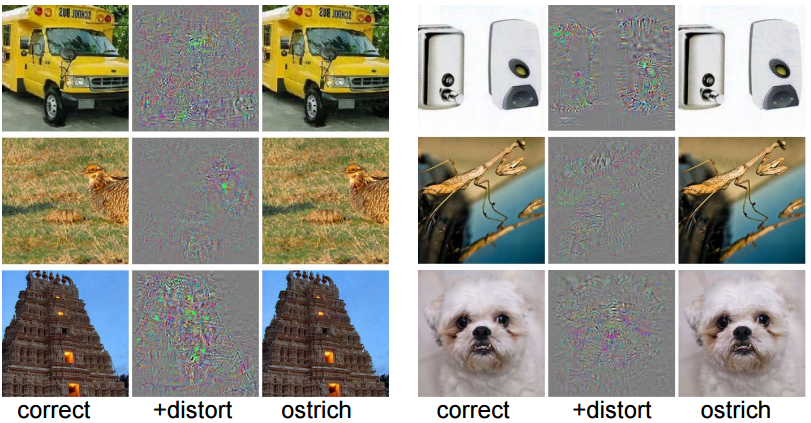
\includegraphics[width=0.65\textwidth]{Images/visualization/14.png}
  \caption{Adversarial data examples}
\end{figure}

The think is that during the forward pass we are applying dot product over all the dimensions of the data (one per pixel) so if we change the input a tiny bit but all in the correct way, the dot product output is going to change a lot.

\begin{figure}[h]
  \centering
  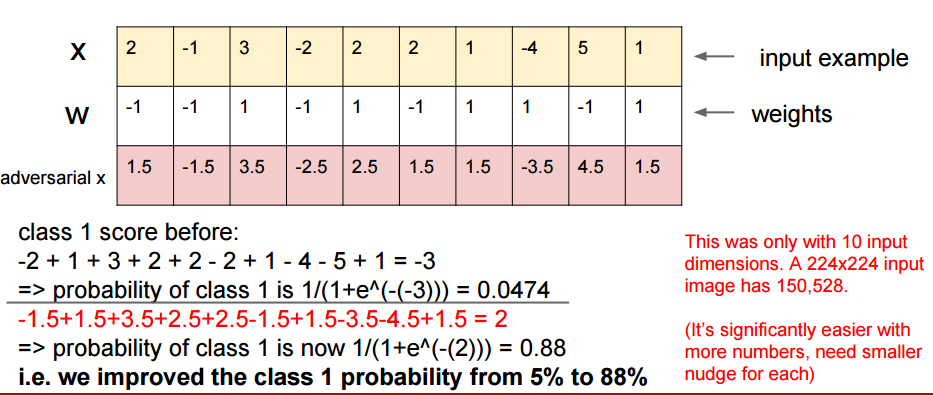
\includegraphics[width=0.8\textwidth]{Images/visualization/15.png}
  \caption{Adversarial data case example}
\end{figure}

This is not a problem of deep learning, its is a problem in learning in general. There are some ways of decreasing this effect. One is to train also with adversarial examples; it will be more robust to them but the classifier accuracy will decrease. Another one is to instead of classifying the hole image, classify chunks.

\part{Layers}
\chapter{Input Layer}
The input layer (that contains the image) should be divisible by 2 many times. Common numbers include 32 (e.g. CIFAR-10), 64, 96 (e.g. STL-10), or 224 (e.g. common ImageNet ConvNets), 384, and 512.
\chapter{Convolutional layer}

\subsection*{Structure}

\begin{itemize}
\item Accepts a volume of size $W_1 \times H_1\times D_1$
\item Requires four hyperparameters:
\begin{itemize}
    \item Number of filters $K$
    \item their spatial extent $F$
    \item the stride $S$
    \item the amount of zero padding $P$
\end{itemize}
\item Produces a volume of size  $W_2 \times H_2 \times D_2$  where:
\begin{itemize}
    \item $W_2 = \frac{W_1-F+2P}{S+1}$
    \item $H_2 = \frac{H_1-F+2P}{S+1}$
    \item $D_2 = K$
\end{itemize}
\item With parameter sharing, it introduces $FFD_1$ weights per filter, for a total of $FFD_1K$ weights and $K$ biases.
\item The filters depth is always equal to the input volume depth.
\item The output volume depth is equal to the number of filters
\item In the output volume, the d-th depth slice (of size $W_2 \times H_2$ is the result of performing a valid convolution of the d-th filter over the input volume with a stride of $S$, and then offset by d-th bias.
\item Normally, in the same conv layer, all filters have the same dimensions so that special optimized routines can be invoked.
\end{itemize}

\subsection*{Explanation}
In a convolution layer we have filters. Each filter is a weight matrix which is convoluted over the input volume. Each time the filter is applied it outputs a single value. The result of convolving the filter over all the input volume is another volume called activation map. A filter's depth is always equal to the input volume depth. You can imagine a filter as a neuron.

\begin{figure}[h]
  \centering
  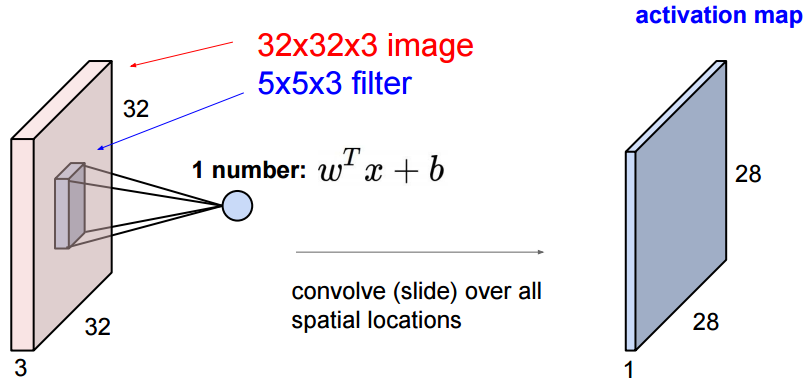
\includegraphics[width=0.4\textwidth]{Images/conv_layer/1.png}
  \caption{Convolution filter}
\end{figure}

Instead of having only one filter, we have a stack of filter which produce a stack of activation maps (one for each filter). In this example this conv layer has a stack of 6 filters ($5 \times 5 \times 3$). All positions in the same activation map share the same weights (filter)

\begin{figure}[h]
  \centering
  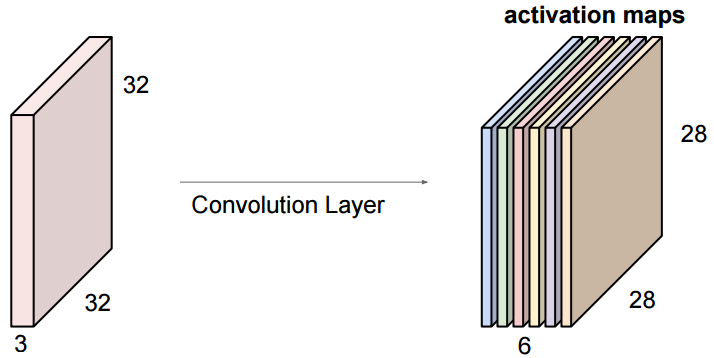
\includegraphics[width=0.4\textwidth]{Images/conv_layer/2.png}
  \caption{6 convolution filters output}
\end{figure}

\begin{figure}[h]
  \centering
  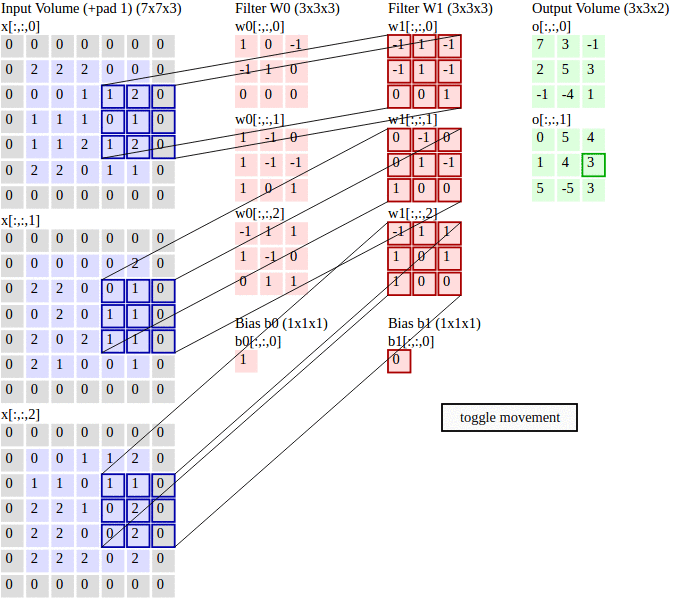
\includegraphics[width=0.5\textwidth]{Images/conv_layer/5.png}
  \caption{Example of a conv layer with 2 filters ($3 \times 3 \times 3$) over an input volume of ($7 \times 7 \times 3$) with 1 padding, which produces and output map of ($3 \times 3 \times 2$)}
\end{figure}

\begin{figure}[h]
  \centering
  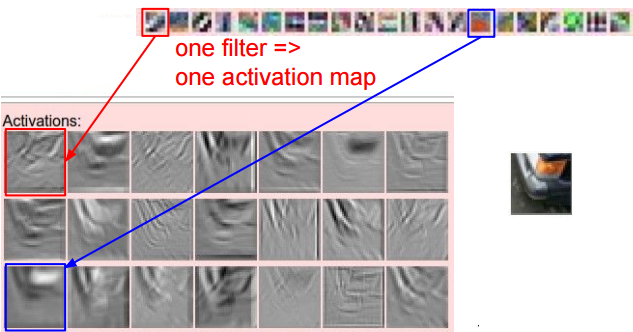
\includegraphics[width=0.4\textwidth]{Images/conv_layer/3.png}
  \caption{Example of the activation maps produced in a convolution layer. The small images on top are the stack of filters, the image on the right the input volume, and the grey-scale images the activation maps. White corresponds to high activations and black to low activations. Notice for example, that the filter marked in blue has an orange part, so when you slide this filter through the input image there are a lot of high activations in the area corresponding to the orange part of the input image. The output of this convolutional layer is going to be a stack of all these activation matrices.}
\end{figure}

\paragraph*{Padding} Add zeros around the input volume. The output volume decreases after each conv layer, so if we would not pad, the size of the activation maps will decrease very fast and after a few layers the volume would be $1 \times 1 \times ?$. This behavior is not desired because in deep learning we want to have a lot of layers. Why padding with zeros and not an extension of the image for example? Because in this way the padded cells do not contribute to the filter.

\paragraph*{Choosing hyperparameters} Should be using small filters (e.g. $3 \times 3$ or at most $5 \times 5$), using a stride of $S=1$, and crucially, padding the input volume with zeros in such way that the conv layer does not alter the spatial dimensions of the input. A common setting of the hyperparameters are: $F=3,S=1,P=1$; $F=5,S=1,P=2$; $F=5,S=2,P=?$and $F=1,S=1,P=0$. $K$ is usually a power of two value (e.g. 32,64,128,512) because libraries normally have optimized routines. If you must use bigger filter sizes (such as $7 \times 7$ or so), it is only common to see this on the very first conv layer that is looking at the input image. For a general $F$, it can be seen that $P=(F-1)/2$ preserves the input size.

\paragraph*{Parameter sharing} In an activation map, all the positions (neurons) share the same weights (filter). It makes sense to share weights because for example if the filter is searching for edges, it makes sense that it search edges in all the image. Moreover, sharing weights spatially avoids over-fitting the filter. It also helps reducing the number of parameters.

\paragraph*{Backpropagation} The backward pass for a convolution operation (for both the data and the weights) is also a convolution (but with spatially-flipped filters). This is easy to derive in the 1-dimensional case with a toy example (not expanded on for now).

\paragraph*{$1 \times 1$ convolution} As an aside, several papers use $1 \times 1$ convolutions, as first investigated by Network in Network. Some people are at first confused to see $1 \times 1$ convolutions especially when they come from signal processing background. Normally signals are 2-dimensional so $1 \times 1$ convolutions do not make sense (it’s just pointwise scaling). However, in ConvNets this is not the case because one must remember that we operate over 3-dimensional volumes, and that the filters always extend through the full depth of the input volume. For example, if the input is [$32 \times 32 \times 3$] then doing $1 \times 1$ convolutions would effectively be doing 3-dimensional dot products (since the input depth is 3 channels).

\paragraph*{Dilated convolutions} A recent development (e.g. see paper by Fisher Yu and Vladlen Koltun) is to introduce one more hyperparameter to the CONV layer called the dilation. So far we’ve only dicussed CONV filters that are contiguous. However, it’s possible to have filters that have spaces between each cell, called dilation. As an example, in one dimension a filter w of size 3 would compute over input x the following: \texttt{w[0]*x[0] + w[1]*x[1] + w[2]*x[2]}. This is dilation of 0. For dilation 1 the filter would instead compute \texttt{w[0]*x[0] + w[1]*x[2] + w[2]*x[4]}; In other words there is a gap of 1 between the applications. This can be very useful in some settings to use in conjunction with 0-dilated filters because it allows you to merge spatial information across the inputs much more agressively with fewer layers. For example, if you stack two 3x3 CONV layers on top of each other than you can convince yourself that the neurons on the 2nd layer are a function of a $5 \times 5$ patch of the input (we would say that the effective receptive field of these neurons is $5 \times 5$). If we use dilated convolutions then this effective receptive field would grow much quicker.

\subsection*{The power of small filters}
\begin{figure}[h]
  \centering
  \includegraphics[width=0.5\textwidth]{Images/conv_layer/4.png}
  \caption{Network in network}
\end{figure}

3 Conv layers of $3 \times 3$ filters have the same receptive field as a 1 Conv layer of $7 \times 7$ filters. But lets compare both options:

Suppose input is $H \times W \times C$ and we use convolutions with $C$ filters to preserve depth (stride 1, padding to preserve $H$, $W$)

\begin{itemize}
\item three CONV with $3 \times 3$ filters
\begin{itemize}
\item Number of weights: $3 \times C \times (3 \times 3 \times C) = 27C^2$
\item Number of multiply-adds: $3 \times (H \times W \times C) \times (3 \times 3 \times C) = 27 HWC^2$
\end{itemize}
\item one CONV with $7 \times 7$ filters
\begin{itemize}
\item Number of weights: $C \times (7 \times 7 \times C) = 49C^2$
\item Number of multiply-adds: $(H x\times W \times C) \times (7 \times 7 \times C) = 49HWC2$
\end{itemize}
\end{itemize}


So 3 Conv layers of $3 \times 3$ filters have the same receptive field of a larger Conv layer of $7 \times 7$ filters but have a lower computation and memory complexity. Moreover, if we have ReLU layers after each Conv layer the 3 Conv layer option is more nonlinear (good).

Lets get crazy. ResNet and GoogLeNet go one step further and use 1x1 filters all over the place to even reduce further the number of parameters. This is commonly known as "Network in Network"


\chapter{Pooling layer}

\subsection*{Structure}

\begin{itemize}
\item Accepts a volume of size

\item Requires two hyperparameters: $W_1 \times H_1 \times D_1$
\begin{itemize}
    \item their spatial extent $F$
    \item the stride $S$
\end{itemize}
\item Produces a volume of size  where: $W_2 \times H_2 \times D_2$
\begin{itemize}
\item $W_2 = \frac{W_1-F}{S}+1$
\item $H_2 = \frac{H_1-F}{S}+1$
\item $D_2 = D_1$
\end{itemize}
\item Introduces zero parameters since it computes a fixed function of the input
\item Note that it is not common to use zero-padding for Pooling layers
\item Has \textbf{NO} parameters
\end{itemize}

\subsection*{Explanation}
It is common to periodically insert a Pooling layer in-between successive Conv layers in a ConvNet architecture. Its function is to progressively reduce the spatial size of the representation to reduce the amount of parameters and computation in the network, and hence to also control overfitting.  This down sampling operations happens on each activation map independently and the volume depth is preserved. The most common way of pooling is max pooling, another one is average pooling but it does not work that well.

The most common form is a pooling layer with filters of size $2 \times 2$ applied with a stride of $2$ downsamples every depth slice in the input by 2 along both width and height, discarding 75\% of the activations. Every MAX operation would in this case be taking a max over $4$ numbers (little $2 \times 2$ region in some depth slice). The depth dimension remains unchanged.

Notice that the pooling layer has NO parameters!!

\begin{figure}[h]
  \centering
  \includegraphics[width=0.4\textwidth]{Images/pool_layer/1.png}
  \caption{ In this example, the input volume of size [$224 \times 224 \times 64$] is pooled with filter size $2$, stride $2$ into output volume of size [$112 \times 112 \times 64$]. Notice that the volume depth is preserved.}
\end{figure}

\begin{figure}[h]
  \centering
  \includegraphics[width=0.45\textwidth]{Images/pool_layer/2.png}
  \caption{The most common downsampling operation is max, giving rise to max pooling, here shown with a stride of $2$. That is, each max is taken over $4$ numbers (little $2 \times 2$ square).}
\end{figure}



\paragraph*{Choosing hyperparameters} There are 2 common setting of the hyperparameters. $F=2, S=2$ that this discards exactly 75\% of the activations in an input volume (due to downsampling by 2 in both width and height). Another slightly less common setting is t. It is very uncommon to see receptive field sizes for max pooling that are larger than 3 because the pooling is then too lossy and aggressive. This usually leads to worse performance.

\paragraph*{Backpropagation} Recall from the backpropagation chapter that the backward pass for a $\text{max}(x, y)$ operation has a simple interpretation as only routing the gradient to the input that had the highest value in the forward pass. Hence, during the forward pass of a pooling layer it is common to keep track of the index of the max activation (sometimes also called the switches) so that gradient routing is efficient during backpropagation.

\paragraph*{Getting rid of pooling} Many people dislike the pooling operation and think that we can get away without it. For example, Striving for Simplicity: The All Convolutional Net proposes to discard the pooling layer in favor of architecture that only consists of repeated CONV layers. To reduce the size of the representation they suggest using larger stride in CONV layer once in a while. Discarding pooling layers has also been found to be important in training good generative models, such as variational autoencoders (VAEs) or generative adversarial networks (GANs). It seems likely that future architectures will feature very few to no pooling layers.
\chapter{Batch Normalization layer}

You have a minibatch of data and you are taking it through your network. You have inserted batch normalization layers through the layer which take your input $x$ and make sure that every feature dimension across the batch you have unit gaussian activations.

\subsection*{Basic Idea}

Batch normalization potentially helps in two ways: faster learning and higher overall accuracy. The improved method also allows you to use a higher learning rate, potentially providing another boost in speed.

Why does this work? Well, we know that normalization (shifting inputs to zero-mean and unit variance) is often used as a pre-processing step to make the data comparable across features. As the data flows through a deep network, the weights and parameters adjust those values, sometimes making the data too big or too small again - a problem the authors refer to as "internal covariate shift". By normalizing the data in each mini-batch, this problem is largely avoided.

Basically, rather than just performing normalization once in the beginning, you're doing it all over place. Of course, this is a drastically simplified view of the matter (since for one thing, I'm completely ignoring the post-processing updates applied to the entire network), but hopefully this gives a good high-level overview.

Adding batch normalization normally slows 30\%.

\subsection*{Extended explanation}

So image you have $N$ samples in your minibatch and D \texttt{features / neuron\_activations} at some points. So this matrix of $X$ is the input to the batch normalization layer. Evaluates empirical mean and variance along every feature. So it makes sure that each column of $X$ is a unit gaussian. You can do this because its perfectly fine to transform it to unit Gaussian because it is differentiable so  you can backpropagate.

\begin{figure}[h]
  \centering
  \includegraphics[width=0.55\textwidth]{Images/bn_layer/1.png}
  \caption{Compute empirical mean and variance for each dimension}
\end{figure}


So what you usually have are fully connected or convoluational layers followed by batch normalization layer before the non-linearity. So they ensure that everything is roughly unit Gaussian at each step of the neural net. One problem is that its not clear that tanh wants exactly unit Gaussian. Because you what tanh to be able to make its outputs more or less defused (more or less saturated) so right now it would not be able to do that.

\begin{figure}[h]
  \centering
  \includegraphics[width=0.55\textwidth]{Images/bn_layer/2.png}
  \caption{In network}
\end{figure}

To solve this you do not only normalize $X$ but you also allow the network to shift by gamma and add $B$. So after you have centred your data you are allowing the network through the backprop to shift and scale the distribution. Also note that the network can learn to undo this layer (it can learn to have the batch normalization layer to be an identity)

\begin{figure}[h]
  \centering
  \includegraphics[width=0.55\textwidth]{Images/bn_layer/3.png}
  \caption{Equations}
\end{figure}

\begin{figure}[h]
  \centering
  \includegraphics[width=0.55\textwidth]{Images/bn_layer/4.png}
  \caption{Algorithm}
  \label{fig:bn_layer_algorithm}
\end{figure}


[2 good (from fig \ref{fig:bn_layer_algorithm})] As you are swiping through different choices of initialization values with and without batch norm you'll see a huge difference. With batch norm it will work with much bigger settings of the initial scale so you don't have to worry as much, it really helps.

[3 good (from fig \ref{fig:bn_layer_algorithm})] It acts somehow as a way of regularization because with batch norm when you have some kind of input $x$ and it goes through the network its representation in some layer of the network is basically not only function of it but also whatever other examples are with $x$ in the batch. Normally all examples are processed independently in parallel, but batch norm tides them together and so your representation at some layer is a function on whatever batch you happen to be sampled in at what it does is to jigger your place in the representation space in that layer. Which is a nice regularizer effect.

\textbf{During testing it works a little different}. During test you what this to be a deterministic function. $\mu$ and $\sigma$ are the once that you used during training. 

\begin{figure}[h]
  \centering
  \includegraphics[width=0.55\textwidth]{Images/bn_layer/5.png}
  \caption{During testing it works a little different}
\end{figure}

\chapter{Upsampling Layer (``Transposed Convolution")}
\subsection*{Learnable Upsampling}

\begin{figure}[h]
  \centering
  \includegraphics[width=0.5\textwidth]{Images/upsampling_layer/1.png}
  \caption{From the paper: ``Fully Convolutional Networks for Semantic Segmentation"}
\end{figure}



\subsection*{Transposed Convolution}
Transposed convolutions -- also called fractionally strided convolutions -- work by swapping the forward and backward passes of a convolution. One way to put it is to note that the kernel defines a convolution, but whether it’s a direct convolution or a transposed convolution is determined by how the forward and backward passes are computed.

The transposed convolution is implemented as the backward pass of a  corresponding non-transposed convolution. It can be thought of as dilating  the input (by adding ``stride - 1" zeros between adjacent input elements),  padding it with the needed number of zeros so it is not out. And then, apply the convolution with the filter flipped 180 degrees.

\begin{figure}[h]
  \centering
  \includegraphics[width=0.4\textwidth]{Images/upsampling_layer/5.png}
  \caption{\textbf{Left}: Visually, for a transposed convolution with stride one and no padding, we just pad the original input (blue entries) with zeroes (white entries). \textbf{Right}: Stride two and padding, the transposed convolution would look like this
}
\end{figure}

\subsection*{Skip Connections}

\begin{figure}[h]
  \centering
  \includegraphics[width=0.8\textwidth]{Images/upsampling_layer/4.png}
  \caption{Skip Connections}
\end{figure}

\chapter{Fully Connected Layer}
FC layers, also called affine layers, produce the high-level reasoning in the DNN. Neurons in a fully connected layer have full connections to all activations in the previous layer, as in regular Neural Networks. Their activations can hence be computed with a matrix multiplication followed by a bias offset.
\chapter{Highway Layer}
A Highway Layer is a type of Neural Network layer that uses a gating mechanism to control the information flow through a layer. Stacking multiple Highway Layers allows for training of very deep networks. Highway Layers work by learning a gating function that chooses which parts of the inputs to pass through and which parts to pass through a transformation function, such as a standard affine layer for example. The basic formulation of a Highway Layer is \texttt{T * h(x) + (1 - T) * x}, where $T$ is the learned gating function with values between $0$ and $1$, $h(x)$ is an arbitrary input transformation and $x$ is the input. Note that all of these must have the same size.




\part{Networks}
\chapter{Recurrent Neural Networks (RNN)}

A recurrent neural network (RNN) is a class of artificial neural network where connections between units form a directed cycle. This creates an internal state of the network which allows it to exhibit dynamic temporal behavior. Unlike feedforward neural networks, RNNs can use their internal memory to process arbitrary sequences of inputs. This makes them applicable to tasks such as unsegmented connected handwriting recognition or speech recognition.

\begin{figure}[h]
  \centering
  \includegraphics[width=0.4\textwidth]{Images/recurrent_neural_networks/1.png}
  \caption{RNN}
\end{figure}

Notice that the same function and the same set of parameters are used at very time step!
We can not have RNNs of enormous length because we have to store in memory the hidden state of each time step to be able to back-propagate. Normally we will have RNNs of max ~25 length.  To process bigger sequences we will divide the sequence in chunks of ~25 and the last hidden state of a chunk is the initial hidden state of the next chunk.

Let's see some wire examples (fig~\ref{fig:rnn_examples}):
\begin{figure}[h]
  \centering
  \includegraphics[width=0.8\textwidth]{Images/recurrent_neural_networks/2.png}
  \caption{RNN examples}
  \label{fig:rnn_examples}
\end{figure}
\begin{enumerate}
\item Vanilla Neural Networks
\item Image Captioning (image to sequence of words)
\item Sentiment Classification (sequence of words to sentiment)
\item Machine Translation (seq of words to seq of words)
\item Video classification on frame level
\end{enumerate}

We can stack RNNs together to produce deeper RNN. In figure \ref{fig:RNN_toghether} case we have stack 3 RNNs. It still works the same as before but now we have 3 weights.
\begin{figure}[h]
  \centering
  \includegraphics[width=0.3\textwidth]{Images/recurrent_neural_networks/4.png}
  \caption{Stacked RNNs}
\end{figure}

\subsection*{Practical Example}

Lets create a RNN that given a sequence of characters predicts the next one. The output is always the prob of each letter in the vocabulary to be the next character:
\begin{itemize}
\item Vocabulary: [h,l,e,o]
\item Example training sequence: "hello"
\end{itemize}

For this example we will use a Vanilla RNN:
\begin{equation}
h_t = \tanh(W_{hh}h_{t-1}+W_{xh}x_t)
\end{equation}
\begin{equation}
y_t = W_{hy}h_{t}
\end{equation}
\begin{equation}
h_0 = 0
\end{equation}

\begin{figure}[h]
  \centering
  \includegraphics[width=0.5\textwidth]{Images/recurrent_neural_networks/10.png}
  \caption{Practical example. You can see this blue boxes being softmax classifier, in other words, at each time step there is a softmax classifier.}
  \label{fig:RNN_toghether}
\end{figure}

A 100 lines of code implementation of a character recognition in python is implemented here:
https://gist.github.com/karpathy/d4dee566867f8291f086

\subsection*{Image Captioning}
Example using RNN for image captioning
\begin{figure}[h]
  \centering
  \includegraphics[width=0.5\textwidth]{Images/recurrent_neural_networks/6.png}
  \caption{"Deep Visual-Semantic Alignments for Generating Image Descriptions", Karpathy and Fei-Fei}
\end{figure}

\section{LSTM}
Normally we will not use Vanilla RNNs, instead, all papers use LSTM. It is very similar, it stills take into account the input and the last state but now the combination of both is more complex and works better. With RNN we have one vector $h$ at each time step. But with LSTM we have two vectors at each time step $h_t$ and $c_t$. Moreover in RNNs the repeating module only has one layer, \textit{tanh}. Instead, LSTM has four.

\begin{figure}[ht]
  \centering
  \includegraphics[width=0.65\textwidth]{Images/recurrent_neural_networks/18.png}
  \caption{\textbf{Left}: RNN with h(green), \textbf{Right}: LSTM with h(hidden vector, green) and c (cell state vector, yellow) }
\end{figure}

\subsection*{How do they work?}
\begin{figure}[h]
  \centering
  \includegraphics[width=0.65\textwidth]{Images/recurrent_neural_networks/9.png}
  \caption{LSTM first equation diagram}
\end{figure}
 where:
\begin{itemize}
\item $c$ cells. Are best though as counters
\item $h$ hidden states
\item $h_t^{l-1}$ vector from below of size $n \times 1$ ($x$ in the figure)
\item $h_{t-1}^{l}$ vector from before of size $n \times 1$ ($h$ in the figure)
\item $i \in [0,1]$ to chose if we want to add, or not, to a cell
\item $f \in [0,1]$ forget gate to reset cells to $0$
\item $o \in [0,1]$ to choose which cells are used to produce
\item $g \in [-1,1]$ to add $-1$ or $1$ to a cell
\end{itemize}

The key to LSTMs is the cell state, the horizontal line running through the top of the diagram. The cell state is kind of like a conveyor belt. It runs straight down the entire chain, with only some minor linear interactions. It’s very easy for information to just flow along it unchanged. The LSTM does have the ability to remove or add information to the cell state, carefully regulated by structures called gates.

Think of $i,f,o$ as boolean variables, we want them to have an interpretation like a gate. They a result of a sigmoid to make them differentiable. They allow us to reset and add to counters, as well as to choose what cells should be used to update $h^l_t$. We can do two operations to cells (counters):
\begin{itemize}
\item reset them with $f \odot c^l_{t-1}$
\item add -1 or 1 with $i \odot g$
\item choose what cells should be used with $o$ to update $h^l_t$: $o \odot \tanh(c^l_t)$
\end{itemize}

\begin{figure}[h]
  \centering
  \includegraphics[width=0.65\textwidth]{Images/recurrent_neural_networks/24.png}
  \caption{LSTM diagram}
\end{figure}

\subsubsection*{Step by step}
\paragraph*{First} Decide what information we’re going to throw away from the cell state. This decision is made by a sigmoid layer called the ``forget gate layer.” It looks at $h_{t−1}$ and $x_t$, and outputs a number between $0$ and $1$ for each number in the cell state $C_{t−1}$. A $1$ represents ``completely keep this” while a $0$ represents ``completely get rid of this.” For example, in a language model trying to predict the next word based on all the previous ones the cell state might include the gender of the present subject, so that the correct pronouns can be used. When we see a new subject, we want to forget the gender of the old subject.

\begin{figure}[h]
  \centering
  \includegraphics[width=0.65\textwidth]{Images/recurrent_neural_networks/20.png}
  \caption{First, decide what information we’re going to throw away from the cell state}
\end{figure}

\paragraph*{Second} Decide what new information we’re going to store in the cell state. This has two parts. First, a sigmoid layer called the ``input gate layer” decides which values we’ll update. Next, a \textit{tanh} layer creates a vector of new candidate values, $\widetilde{C}_t$, that could be added to the state. In the next step, we’ll combine these two to create an update to the state. For example, in the example of our language model, we’d want to add the gender of the new subject to the cell state, to replace the old one we’re forgetting.

\begin{figure}[h]
  \centering
  \includegraphics[width=0.65\textwidth]{Images/recurrent_neural_networks/21.png}
  \caption{Second, decide what information we’re going to store in the cell state}
\end{figure}

\paragraph*{Third} Update the old cell state, $C_{t−1}$, into the new cell state CtCt. The previous steps already decided what to do, we just need to actually do it. We multiply the old state by $f_t$, forgetting the things we decided to forget earlier. Then we add $i_t∗\widetilde{C}_t$. This is the new candidate values, scaled by how much we decided to update each state value. In the case of the language model, this is where we’d actually drop the information about the old subject’s gender and add the new information, as we decided in the previous steps.

\begin{figure}[h]
  \centering
  \includegraphics[width=0.65\textwidth]{Images/recurrent_neural_networks/22.png}
  \caption{Third, update the old cell state}
\end{figure}

\paragraph*{Fourth} Finally, we cide what we’re going to output. This output will be based on our cell state, but will be a filtered version. First, we run a sigmoid layer which decides what parts of the cell state we’re going to output. Then, we put the cell state through \textit{tanh} (to push the values to be between $−1$ and $1$) and multiply it by the output of the sigmoid gate, so that we only output the parts we decided to. For the language model example, since it just saw a subject, it might want to output information relevant to a verb, in case that’s what is coming next. For example, it might output whether the subject is singular or plural, so that we know what form a verb should be conjugated into if that’s what follows next.

\begin{figure}[h]
  \centering
  \includegraphics[width=0.65\textwidth]{Images/recurrent_neural_networks/23.png}
  \caption{Fourth, decide what we’re going to output}
\end{figure}

\subsection*{Variants on LSTMs}
But not all LSTMs are the same as the above. In fact, it seems like almost every paper involving LSTMs uses a slightly different version. The differences are minor, but it’s worth mentioning some of them. Greff, et al. (2015) do a nice comparison of popular variants, finding that they’re all about the same.

\begin{figure}[h]
  \centering
  \includegraphics[width=0.65\textwidth]{Images/recurrent_neural_networks/25.png}
  \caption{One popular LSTM variant, introduced by Gers \& Schmidhuber (2000), is adding ``peephole connections.” This means that we let the gate layers look at the cell state. The diagram adds peepholes to all the gates, but many papers will give some peepholes and not others.}
\end{figure}

\begin{figure}[h]
  \centering
  \includegraphics[width=0.65\textwidth]{Images/recurrent_neural_networks/26.png}
  \caption{Another variation is to use coupled forget and input gates. Instead of separately deciding what to forget and what we should add new information to, we make those decisions together. We only forget when we’re going to input something in its place. We only input new values to the state when we forget something older.}
\end{figure}

\begin{figure}[h]
  \centering
  \includegraphics[width=0.65\textwidth]{Images/recurrent_neural_networks/27.png}
  \caption{A slightly more dramatic variation on the LSTM is the Gated Recurrent Unit, or GRU, introduced by Cho, et al. (2014). It combines the forget and input gates into a single ``update gate.” It also merges the cell state and hidden state, and makes some other changes. The resulting model is simpler than standard LSTM models, and has been growing increasingly popular.}
\end{figure}

These are only a few of the most notable LSTM variants. There are lots of others, like Depth Gated RNNs by Yao, et al. (2015). There’s also some completely different approach to tackling long-term dependencies, like Clockwork RNNs by Koutnik, et al. (2014).

\subsection*{Difference between RNN and LSTM}
\begin{figure}[!htb]
  \centering
  \includegraphics[width=0.65\textwidth]{Images/recurrent_neural_networks/19.png}
  \caption{Difference between RNN (\textbf{left}) and LSTM (\textbf{right})}
\end{figure}

\begin{itemize}
\item RNN transformative interaction of the state, LSTM additive interaction of the state.
\item In RNN you are operating and transforming the state vector. So you are changing your hidden state from time step to time step. Instead, LSTM has these cells states flowing through. A subset of cells (or all of them) to compute the hidden state. Then, based on hidden state, we decide how to operate over the cell. We can reset it and/or adding interaction.
\item RNNs look identical to plain nets, LSTMs to ResNets.
\item RNNs has vanishing gradients, so you can not learn dependencies between distant time steps.LSTMs do not have the problem of vanishing gradients. In a video in evernote they introduce gradient noise to a layer and show how it evolves. We can see that RNN automatically kills it while LSTM maintains it more time. This means that RNN can not learn long term relationships.
\end{itemize}

\subsection{Bidirectional RNN}
A Bidirectional Recurrent Neural Network is a type of Neural Network that contains two RNNs going into different directions. The forward RNN reads the input sequence from start to end, while the backward RNN reads it from end to start. The two RNNs are stacked on top of each others and their states are typically combined by appending the two vectors. Bidirectional RNNs are often used in Natural Language problems, where we want to take the context from both before and after a word into account before making a prediction.


\section*{Summary}
\begin{itemize}
\item RNNs allow a lot of flexibility in architecture design
\item Vanilla RNNs are simple but don’t work very well
\item Common to use LSTM or GRU: their additive interactions improve gradient flow
\item Backward flow of gradients in RNN can explode or vanish. Exploding is controlled with gradient clipping. Vanishing is controlled with additive interactions (LSTM)
\item Better/simpler architectures are a hot topic of current research
\item Better understanding (both theoretical and empirical) is needed.
\end{itemize}


 
\chapter{Autoencoders}
The idea of autoencoders is that we want to force a network to try to reconstruct our data and hopefully it will learn a useful representation of the data. For traditional autoencoders this is use for feature learning and for variational atoencoders to generate fake samples.

\section{Traditional Autoencoder}
\begin{figure}[!htb]
  \centering
  \includegraphics[width=0.45\textwidth]{Images/autoencoders/1.png}
  \caption{Traditional Autoencoder}
\end{figure}

Normally encoder will be a 4-layer conv, and the decoder a 4-layer upconv. Sometimes they share weights (in fact they are the same, we only have to transpose them): $\dim(x) = D, \dim(z)=H$, $w_e : H \times D, w_d : D \times H = w_e^T$.

The idea is to pass the input data through an encoder network that will produce features $z$. This step can be thought as PCA. We are transforming the input data and transforming it into another feature representation. The encoder network is usually a ReLU CNN. Normally $z$ is smaller than $x$ (dimensionality reduction).

The problem is that we do not have any explicit labels to use to know which information is relevant and which one its not to decide how to make the dimensionality reduction. To decide which is the most relevant data we reconstruct the input data only with the information in the $z$ features and compare the reconstruction with the original image.

Specially if the $z$ features are small, hopefully, it will force the network to summarize the useful statistics and to discover useful features of the input image.



\subsection*{How do we train them?}
\begin{figure}[!htb]
  \centering
  \includegraphics[width=0.35\textwidth]{Images/autoencoders/2.png}
  \caption{Traditional Autoencoder}
\end{figure}
Normally it is trained as a regular NN with euclidean distance as the loss function comparing the input data vs the reconstructed data. 

Normally, after training, the decoder will be thrown away.


\subsection*{Unsupervised + Supervised learning}
\begin{figure}[!htb]
  \centering
  \includegraphics[width=0.4\textwidth]{Images/autoencoders/3.png}
  \caption{Traditional Autoencoder}
\end{figure}
The idea is first to train the network with unsupervised data, and then fine tune with a small labeled dataset. This idea is beautiful in the sense that we could train our networks with millions of unlabeled data from the internet, and the fine tune the network with a labeled dataset such us KITTI. The problem is that is yet not working that well.

\section{Variational Autoencoder}
Transforming traditional autoencoders to Bayesian, allows us to generate data.

\begin{figure}[!htb]
  \centering
  \includegraphics[width=0.3\textwidth]{Images/autoencoders/4.png}
  \caption{Variational Autoencoder}
\end{figure}

We assume that it exists a distribution with parameters $\phi^*$ that is generating the latent states $z$ from $x$ (given $x$ we can sample $z$): $q_{\phi^*}(z|x)$

We also assume a conditional distribution with parameters $\theta^*$ that given the latent states we can sample $x$: $p_{\theta^*}(x|z^{(i)})$

We assume that these distributions are diagonal Gaussian and we will try to approximate them with two neural nets with parameters $\phi$ and $\theta$. Also, we assume $p_{\theta^*}(z)$ unit Gaussian. We could assume more fancy distributions, but we use these ones because they are easy to work with.

\begin{enumerate}
\item Input data $x$
\item Pass $x$ through the encoder network which will spit out a distribution of the latent states $z$ ( the mean and (diagonal) covariance of $q_{\phi}(z|x)$).
\item Sample latent states of high probability from the obtained distribution $q_{\phi}(z|x)$ given our input data $x$.
\item Once we have some samples of $z$, pass them trough the decoder which will spit out the distribution of the input data $x$ ( the mean and (diagonal) covariance of $p_{\theta^*}(x|z^{(i)})$)
\item Finally, we can sample data $xx$ of high probability from the obtained distribution $p_{\theta}(x|z)$ given the latent variables $z$. $xx$ should be similar to $x$.
\end{enumerate}

\subsection*{Generate fake data}
We train Variational Autoencoders as a normal autoencoder: reconstruction loss at the end, regularization toward prior in the middle. After the network is trained we can use it to generate fake data.

\begin{enumerate}
\item We first sample from the prior distribution $p_{\theta}(z)$ which we have assumed that it is unit Gaussian so it is really easy to draw random samples from this distribution.
\item Pass a sample through the decoder network which we have trained during tinning. The decoder will spit out a distribution over our data points x in terms of both a mean and covariance
\item Once we have a mean and a covariance, we have a the $p_{\theta}(x|z)$ which is also easy to sample from because we have assume that is diagonal Gaussian. This samples are going to be new fake data $xx$
\end{enumerate}

\begin{figure}[!htb]
  \centering
  \includegraphics[width=0.3\textwidth]{Images/autoencoders/4.png}
  \caption{Generate data with Variational Autoencoder}
\end{figure}

To try figuring out what the decoder network has learn we can densely sample all the latent space.

\begin{figure}[!htb]
  \centering
  \includegraphics[width=0.3\textwidth]{Images/autoencoders/6.png}
  \caption{In this example, the encoder was trained with a latent space of two dimensions. This image was generated by passing each point of this 2D latent space through the decoder. It can be seen that the net has learn to interpolate the digits. For example, we can see 6s transforming to 0s.}
\end{figure}


One of the reasons that is making this nice separation of classes between axes, is that we are assuming diagonal distribution. Thus, we are assuming as a prior to our system that latent variables (axis in the latent space) are independent (there is no relation between them).

\begin{figure}[!htb]
  \centering
  \includegraphics[width=0.25\textwidth]{Images/autoencoders/5.png}
  \caption{Example of dense sampling of the latent space}
\end{figure}

In the CS231n course - lecture 14 there is more information explaining that it is not possible to use maximum likelihood and explaining how to solve this situation.

\subsection*{All together}
A recent paper (Dosovitskiy and Brox, “Generating Images with Perceptual Similarity Metrics based on Deep Networks”, arXiv 2016) proposes a method to mix all together to make the fake images more realistic.
\begin{figure}[!htb]
  \centering
  \includegraphics[width=0.6\textwidth]{Images/autoencoders/11.png}
  \caption{All together to generate better images}
\end{figure}

\section{Overview}
The idea of autoencoders is that we want to force a network to try to reconstruct our data and hopefully it will learn a useful representation of the data. For traditional autoencoders this is use for feature learning and for variational atoencoders to generate fake samples.

\begin{itemize}
\item Traditional Autoencoders
\begin{itemize}
\item Try to reconstruct input
\item Used to learn features, initialize supervised model
\item Not used much anymore
\end{itemize}
\item Variational Autoencoders
\begin{itemize}
\item Bayesian meets deep learning
\item Sample from model to generate images
\end{itemize}
\end{itemize}

\chapter{Generative Adversarial Nets}
A strategy to generate images with less math than Variational Autoencoders.

The idea is to start with a random noise that is normally drawn from a unit Gaussian (or something similar) and we will pass it through a Generator network. The Generator network looks very much like the decoder on the autoencoder and spits fake images. Then, a discriminator network is responsible for deciding/estimating if the input image is fake or a real.

\begin{figure}[!htb]
  \centering
  \includegraphics[width=0.25\textwidth]{Images/gans/8.png}
  \caption{GAN}
\end{figure}

\subsection*{How to we train them?}
\begin{figure}[!htb]
  \centering
  \includegraphics[width=0.5\textwidth]{Images/gans/7.png}
  \caption{GAN}
\end{figure}
We train this network all together. The Generator will receive minibatches of random noise, at it will spit fake images. The Discriminator will receive batches partially fake and real; and it will try to decide which ones are real and which ones are fake.

The generator will improve its fake images by trying to trick the discriminator.



\subsection*{Examples}
Interpolating random noise vectors. In figure \ref{fig:gans1} the images in the left and right extremes are obtained by sampling two random points (vectors) of the $z$ space and passing them through the generative net. Then the interpolation between pairs of extreme images is performed by interpolating the $z$ vectors and passing them through the generative net.
\begin{figure}[!htb]
  \centering
  \includegraphics[width=0.6\textwidth]{Images/gans/9.png}
  \caption{Interpolating random noise vectors}
  \label{fig:gans1}
\end{figure}

Another experiment shows that the generator is learning a useful representation of the data. In this experiment they randomly generated multiple images of faces and then manually organized in the classes "smiling woman", "neutral woman", "neutral man". Then, they produce the mean $z$ average representation of each image and perform the arithmetic operation of z\_{smiling woman}-z\_{neutral woman}+z\_{neutral man} produces a smiling man.

\begin{figure}[!htb]
  \centering
  \includegraphics[width=0.6\textwidth]{Images/gans/10.png}
  \caption{Generator learning a useful representation of the data}
\end{figure}
\chapter{Region Based CNN (R-CNN)}

R-CNN (Region based CNN) are used for object detection. Another network also used for objection detection is YOLO (You only look once)

\section{R-CNN (do not use this method, deprecated)}

\begin{figure}[h]
  \centering
  \includegraphics[width=0.6\textwidth]{Images/region_based_cnn/1.png}
  \caption{R-CNN}
\end{figure}
So the idea for object detection is to use R-CNN. First run a region proposal algorithm to obten regions of interets. Then, warp this regions into a fixed size and run the ConvNet with regression head and classification head. The regression head objective is to output an offset to correct "slightly wrong" region proposals.

R-CNN probelms:
\begin{itemize}
\item Slow at test-time: need to run full forward pass of CNN for each region proposal
\item SVMs and regressors are post-hoc: CNN features not updated in response to SVMs and regressors
\item Complex multistage training pipeline
\end{itemize}


Train a R-CNN

1.- \textbf{Train} (or download) a classification model (e.g. AlexNet).
\begin{figure}[h]
  \centering
  \includegraphics[width=0.6\textwidth]{Images/region_based_cnn/2.png}
  \caption{Train}
\end{figure}
2.- \textbf{Fine-tune model for detection}. Instead of X classes you want Y classes + background. To do so, throw away the final fully-connected layer, add the new one and retrain using positive/negative regions from detection images.
\begin{figure}[h]
  \centering
  \includegraphics[width=0.6\textwidth]{Images/region_based_cnn/3.png}
  \caption{Fine-tune}
\end{figure}
3.- \textbf{Extract features}. Extract region proposals for all images. For each region: warp to CNN input size, run forward through CNN, save last pool features to disk.
\begin{figure}[h]
  \centering
  \includegraphics[width=0.6\textwidth]{Images/region_based_cnn/4.png}
  \caption{Extract features}
\end{figure}
4.- \textbf{Train classification head}. Train one binary SVM per class using as input the saved features from last step.

5- \textbf{Train regression head}. For each class, train a linear regression model to map from cached features to offset to GT boxes to make up for "slightly wrong" proposals of the region proposals.
\begin{figure}[h]
  \centering
  \includegraphics[width=0.6\textwidth]{Images/region_based_cnn/5.png}
  \caption{Train regression head}
\end{figure}
\begin{figure}[h]
  \centering
  \includegraphics[width=0.6\textwidth]{Images/region_based_cnn/6.png}
  \caption{Usual datasets for training}
\end{figure}



\section{Fast R-CNN (do not use this method, deprecated)}
A new proposal called Fast R-CNN appeared trying to solve R-CNN problems. The idea is just to swap the order of extracting regions of interest and features. Still, no sliding windows.

\begin{figure}[h]
  \centering
  \includegraphics[width=\textwidth]{Images/region_based_cnn/10.png}
  \caption{Fast R-CNN training/testing time}
\end{figure}

\subsection*{The only mystery here are region of interest pooling.}

The HxW image is processed by the convolution and pooling part and regions of interest are proposed (with an external algorithm). The problem now is that the FC layer is expecting a fixed size input. To solve this, given the region proposal, we project it onto the conv feature map, divide it into hxw grid and do max-pool within each grid cell.

\begin{figure}[h]
  \centering
  \includegraphics[width=0.6\textwidth]{Images/region_based_cnn/9.png}
  \caption{process}
\end{figure}

With this simple straggly the FC layer will always receive the same input size.  Moreover, we can backprop through this strategy with no problem because it only uses max-pool.

In terms of mAP (accuracy) is more or less the same
The computational time improvement of Fast R-CNN w.r.t. R-CNN is impressive:
\begin{itemize}
\item x8.8 training time speed up
\item x25 testing time speed up (50s to 2s)
\end{itemize}

However, the bottleneck is extracting the regions with a region proposals algorithm. Without it, the speed would be:
\begin{itemize}
\item x146 testing time speed up (47s to 0.32s)
\end{itemize}

so why not extracting the ROIs with the CNN? this is what Faster R-CNN proposes

\section{Faster R-CNN}

To solve the problem of region proposals algorithm botleneck in Fast R-CNN, Faster R-CNN proposes to extract the regions of interest with another network using the information of the last layer of the CNN net.

Insert a Region Proposal Network (RPN) after the last convolutional layer.

RPN trained to produce region proposals directly; no need for
external region proposals!

After RPN, use RoI Pooling and an upstream classifier and bbox regressor just like Fast R-CNN

Still, the Rol pooling does not allow to introduce rotations into your regions of interests. To introduce rotations, a DeepMind paper proposes to do bilinear interpolation similar computer graphics.

\begin{figure}[h]
  \centering
  \includegraphics[width=0.4\textwidth]{Images/region_based_cnn/14.png}
  \caption{Faster R-CNN}
\end{figure}

\subsection*{The cool thing here is the region proposal network, how does it work?}

Build a small network for:

\begin{itemize}
\item Classifying object or no-object, and
\item Regressing bbox locations
\end{itemize}

Use N anchor boxes at each location. Anchors are translation invariant: use the same ones at every location. For all the feature map points, at the original input image apply all anchors to the point corresponding to the current feature map point. So we take as features the convolutional feature map region corresponding to the anchor region in the original image.

For each of this anchor boxes it produces a score weather there is an object or not; and a finer localization with reference to the anchor (they are an offset to the anchor boxes)

So you are learning different weights for each anchor.

\begin{figure}[h]
  \centering
  \includegraphics[width=0.6\textwidth]{Images/region_based_cnn/11.png}
  \caption{The cool thing here is the region proposal network, how does it work?}
\end{figure}

\subsection*{How to train it?}

To train it, in some unpublished work, it trains the net as a net with 4 losses

One network, four losses
\begin{itemize}
\item RPN classification (anchor good / bad)
\item RPN regression (anchor to proposal)
\item Fast R-CNN classification (over classes)
\item Fast R-CNN regression (proposal to box)
\end{itemize}

\begin{figure}[h]
  \centering
  \includegraphics[width=0.6\textwidth]{Images/region_based_cnn/15.png}
  \caption{How to train it?}
\end{figure}

In terms of mAP (accuracy) is more or less the same than with Fast R-CNN
The computational time improvement of Faster R-CNN w.r.t. R-CNN is impressive: x250 testing time speed up (50s to 0.2s)


\chapter{YOLO}
YOLOs are used for object detection. Other networks also used for objection detection are R-CNN, Fast R-CNN \& Faster R-CNN.

\begin{figure}[h]
  \centering
  \includegraphics[width=0.5\textwidth]{Images/yolo/1.png}
  \caption{YOLO}
\end{figure}

Another detection strategy that is also commonly used is YOLO. The idea is to solve detection as only a regression problem. Direct prediction using a CNN.

Divide image into $S \times S$ grid, they use $S = 7$. The, within each grid cell predict:
\begin{itemize}
\item $B$ boxes: 4 coordinates + confidence, they use $B = 2$
\item Class scores: $C$ numbers
\end{itemize}

Regression from input image to output $S \times S \times (5*B+C)$ tensor.

It can go at real-time at the expense of lower mAP than Faster R-CNN.
\chapter{RNN ConvNet}
\section*{Local motion}
\begin{figure}[h]
  \centering
  \includegraphics[width=0.6\textwidth]{Images/rnn_convnet/1.png}
  \caption{Getting there}
\end{figure}
\begin{figure}[h]
  \centering
  \includegraphics[width=0.5\textwidth]{Images/rnn_convnet/2.png}
  \caption{Large-scale Video Classification with Convolutional Neural Networks, Karpathy et al., 2014]}
\end{figure}

\section*{Global motion}
Delving Deeper into Convolutional Networks for Learning Video Representations, Ballas et al., 2016
\begin{figure}[h]
  \centering
  \includegraphics[width=0.35\textwidth]{Images/rnn_convnet/3.png}
  \caption{Large-scale Video Classification with Convolutional Neural Networks, Karpathy et al., 2014]}
\end{figure}
\begin{figure}[h]
  \centering
  \includegraphics[width=0.75\textwidth]{Images/rnn_convnet/6.png}
  \caption{The idea is to modify GRU adding convolutions. The Gated Recurrent Unit (GRU) is a simplified version of an LSTM unit with fewer parameters. Just like an LSTM cell, it uses a gating mechanism to allow RNNs to efficiently learn long-range dependency by preventing the vanishing gradient problem. The GRU consists of a reset and update gate that determine which part of the old memory to keep vs. update with new values at the current time step.}
\end{figure}
\begin{figure}[h]
  \centering
  \includegraphics[width=0.65\textwidth]{Images/rnn_convnet/5.png}
  \caption{Original paper diagram}
\end{figure}
\begin{figure}[h]
  \centering
  \includegraphics[width=0.45\textwidth]{Images/rnn_convnet/4.png}
  \caption{A more clear diagram}
\end{figure}

\section*{Summary}
\begin{enumerate}
\item You think you need a Spatio-Temporal Fancy VideoConvNet
\item STOP. Do you really?
\item Okay fine: do you want to model:
\begin{itemize}
\item local motion? (use 3D CONV), or
\item global motion? (use LSTM).
\end{itemize}
\item Try out using Optical Flow in a second stream (can workbetter sometimes)
\item Try out GRU-RCN! (imo best model)
\end{enumerate}

\chapter{Attention Models}
First recall RNN for Captioning. It would be better if it could look the image more than once and focus its attention to specific parts of the image.

\section*{Soft Attention for Captioning}
\begin{figure}[h]
  \centering
  \includegraphics[width=0.7\textwidth]{Images/attention_models/1.png}
  \caption{Soft Attention for Captioning - Xu et al, “Show, Attend and Tell: Neural Image Caption Generation with Visual Attention”, ICML 2015}
\end{figure}

\begin{enumerate}
\item Compute the features with a CNN. Extract not the last ones but from an early layer. This is way it is a grid of features and not a single vector. In this way we have information of the localization of the input image features
\item Use this features to initialize the h0 hidden state
\item Now things get different with respect RNN for captioning. Instead of using h0 to compute distribution over words, we use it to compute a prob distribution over L locations. This would we implemented with a couple of affine layers (= FC) and softmax to give a distribution.
\item We produce a weighted sum of features using the prob distribution over locations. This can be seen as taking the feature vector and summarizing it to a vector. This gives as a weighted features that is used to decide where to focus.
\item The next hidden state has as inputs the past hidden state and a word (like CNN) but now we also add the weighted features.
\item The hidden state is used to produce a prob distribution over words and also a new distribution over locations. These are implemented with a couple of FC layers on top of the hidden state.
\item Go to 4
\end{enumerate}


\section*{Soft vs Hard Attention}
Lets see how this summarization vectors z are produced
\begin{figure}[h]
  \centering
  \includegraphics[width=0.7\textwidth]{Images/attention_models/2.png}
  \caption{Soft Attention vs Hard Attention}
\end{figure}

Both soft and hard attention model produce the same output. Notice that the soft attention is more diffuse because it is averaging prob from the image. And Hard attention it is only focusing in one element.

Hard attention is normally faster at test time because is only focusing on an specific thing at every step instead of looking at big regions of the image.

\begin{figure}[h]
  \centering
  \includegraphics[width=0.7\textwidth]{Images/attention_models/3.png}
  \caption{Example Soft Attention vs Hard Attention}
\end{figure}

Both have the same problem, they are constrained by a grid  over the input image which makes them more blurry. z is not continuous. To work in a continuous way it exists the so called "Spatial Transformed Networks"


\section*{Recap}
Soft attention:
\begin{itemize}
\item Easy to implement: produce distribution over input locations, reweight features and feed as input
\item Attend to arbitrary input locations using spatial transformer networks
\end{itemize}

Hard attention:
\begin{itemize}
\item Attend to a single input location
\item Can’t use gradient descent!
\item Need reinforcement learning (because they are not differentiable)
\end{itemize}
\chapter{Spatial Transformer Networks}

The use of spatial transformers results in models which learn invariance to translation, scale, rotation and more generic warping, resulting in state-of-the-art performance on several benchmarks, and for a number of classes of transformations.

\begin{figure}[h]
  \centering
  \includegraphics[width=0.8\textwidth]{Images/spatial_transformer_networks/2.png}
  \caption{Spatial Transformer Networks}
\end{figure}

We would like a function that given a continuous box coordinates cropped the input image. The problem is that it is not possible to crop in a continuous way because we are constraint, at least, by pixels.

The idea is to have a function that maps output pixels coord to input pixels coord. This function is deferentiable w.r.t the affine parameters $\theta$.

With this function, the network will attend to input regions by predicting $\theta$.

\begin{figure}[h]
  \centering
  \includegraphics[width=0.8\textwidth]{Images/spatial_transformer_networks/1.png}
  \caption{continious coordinates}
\end{figure}

They put the info explained on top row in a self contained module which they call "Spatial Transformer" which is divided in three parts:
\begin{itemize}
\item Localisation net: Outputs the affine parameters $\theta$.
\item Grid Generator: Use $\theta$ to compute the sampling grid
\item Sampler: With bilinear interpolation produces outputs.
\end{itemize}

Notice that all this modules are continuous and differentiable.

\begin{figure}[h]
  \centering
  \includegraphics[width=0.8\textwidth]{Images/spatial_transformer_networks/3.png}
  \caption{Deformation examples}
\end{figure}
\chapter{Famous Networks}
\section*{LeNet-5}
\begin{figure}[h]
  \centering
  \includegraphics[width=0.8\textwidth]{Images/famous_networks/1.png}
  \caption{LeNet}
\end{figure}
The first successful applications of Convolutional Networks were developed by Yann LeCun in 1990’s. Of these, the best known is the LeNet architecture that was used to read zip codes, digits, etc.

\section*{AlexNet}
The first work that popularized Convolutional Networks in Computer Vision was the AlexNet, developed by Alex Krizhevsky, Ilya Sutskever and Geoff Hinton. The AlexNet was submitted to the ImageNet ILSVRC challenge in 2012 and significantly outperformed the second runner-up (top 5 error of 16\% compared to runner-up with 26\% error). The Network had a very similar architecture to LeNet, but was deeper, bigger, and featured Convolutional Layers stacked on top of each other (previously it was common to only have a single CONV layer always immediately followed by a POOL layer). 60M parameters.

\begin{figure}[h]
  \centering
  \includegraphics[width=0.8\textwidth]{Images/famous_networks/2.png}
  \caption{AlexNet. There is an error in the paper figure, the input image must be of 227 so that the rest of volumes are coherent}
\end{figure}

\section*{VGGNet}
The runner-up in ILSVRC 2014 was the network from Karen Simonyan and Andrew Zisserman that became known as the VGGNet. Its main contribution was in showing that the depth of the network is a critical component for good performance. Their final best network contains 16 CONV/FC layers and, appealingly, features an extremely homogeneous architecture that only performs $3 \times 3$ convolutions and $2 \times 2$ pooling from the beginning to the end. Their pretrained model is available for plug and play use in Caffe. A downside of the VGGNet is that it is more expensive to evaluate and uses a lot more memory and parameters (140M). Most of these parameters are in the first fully connected layer, and it was since found that these FC layers can be removed with no performance downgrade, significantly reducing the number of necessary parameters.

The most of the network parameters are in the FC layer and most of the memory required by the network is used in the first 2 ConvLayers.

\begin{figure}[h]
  \centering
  \includegraphics[width=0.8\textwidth]{Images/famous_networks/3.png}
  \caption{VGGNet - 7.3\% top 5 error in ImageNet}
\end{figure}

\section*{GoogLeNet}
The ILSVRC 2014 winner was a Convolutional Network from Szegedy et al. from Google. Its main contribution was the development of an Inception Module that dramatically reduced the number of parameters in the network (4M, compared to AlexNet with 60M). Additionally, this paper uses Average Pooling instead of Fully Connected layers at the top of the ConvNet, eliminating a large amount of parameters that do not seem to matter much. There are also several followup versions to the GoogLeNet, most recently Inception-v4. 
\begin{figure}[h]
  \centering
  \includegraphics[width=0.8\textwidth]{Images/famous_networks/4.png}
  \caption{VGGNet - 6.7\% top 5 error in ImageNet}
\end{figure}
\begin{figure}[h]
  \centering
  \includegraphics[width=0.8\textwidth]{Images/famous_networks/5.png}
  \caption{VGGNet structure}
\end{figure}

\section*{ResNet}
Let $H(x)$ be a function that you desire to obtian. In a typical net you would compute a squence of steps \texttt{ReLu(ReLu(xw1+b1)*w2+b2)} to transform $x$ to $H(x)$. Instead, in a ResNet you compute a delta to be added to the original input to obtain $H(x)$.

What is nice about it is that in \textit{plain nets}, gradients must flow through all the transformations. Instead, in \textit{residual nets} because it is addition (distributes the gradient equally to all its children), the gradient with flow through the (weights, ReLU) but will also skip this transformations and will go directly to the previous part and flow directly to the previous block. So the gradients can skip all the transformations and go directly to the first layer. In this way, you can train very fast the first layer which is doing simple statistics, and the rest of layers will learn to add to the single in between to make it work at the end.

\begin{figure}[h]
  \centering
  \includegraphics[width=0.6\textwidth]{Images/famous_networks/6.png}
  \caption{Plain vs Residual Net}
\end{figure}

\begin{figure}[h]
  \centering
  \includegraphics[width=0.3\textwidth]{Images/famous_networks/7.png}
  \caption{ResNet (much more layers than the ones on the diagram)}
\end{figure}

Another way of seeing it, it that ResNets are only computing a delta on top of the identity. So it makes it nice to optimize.

 Residual Network developed by Kaiming He et al. was the winner of ILSVRC 2015. It features specialskip connections and a heavy use of batch normalization. The architecture is also missing fully connected layers at the end of the network. ResNets are currently by far state of the art Convolutional Neural Network models and are the default choice for using ConvNets in practice (as of May 10, 2016). In particular, also see more recent developments that tweak the original architecture from Kaiming He et al. Identity Mappings in Deep Residual Networks (published March 2016).
It is interesting that after the first layer they do polling (the only polling in all the net) and they scale the input image of $244 \times 244$ to $56 \times 56$, and the net works that well. Its crazy that all the layer (except the first one) work wit $56 \times 56 \times ?$ and even compressing the data this much it has a high accuracy.


\begin{figure}[h]
  \centering
  \includegraphics[width=0.8\textwidth]{Images/famous_networks/9.png}
  \caption{ResNet structure. 3.6\% top 5 error in ImageNet, 152 layers, 2-3 weeks training on 8 GPU machine, faster at test time that VGGNet}
\end{figure}

\section*{Should we add infinite layers?}
In plot \ref{fig:depth_rev} it is clear that networks are getting deeper and deeper
\begin{figure}[h]
  \centering
  \includegraphics[width=0.4\textwidth]{Images/famous_networks/10.png}
  \caption{Depth revolution}
  \label{fig:depth_rev}
\end{figure}
But we have to be careful. Plot \ref{fig:cifar_train_error} shows CIFAR-10 training error. In the left plain nets (weighted layer + ReLU) in the right ResNet. How it is possible to get a higher training error (dashed lines) with higher number of layers? It should not happen, the model is more complex. The explanation is that we are still not capable of optimizing them good enough.

\begin{figure}[h]
  \centering
  \includegraphics[width=0.8\textwidth]{Images/famous_networks/11.png}
  \caption{CIFAR-10 training error}
  \label{fig:cifar_train_error}
\end{figure}

However, ResNets always improve the test and training error.

So the answer to the question is that we should keep adding more layers but not in a naive way, we should do it in a ResNet way 

\part{Applications}
\chapter{Applications}
\begin{figure}[h]
  \centering
  \includegraphics[width=0.55\textwidth]{Images/applications/1.png}
  \caption{Some applications examples}
\end{figure}

\section{Classification}
Train a classification model with softmax loss. The input is the entire image and the output are C probabilities (one per class) of being in the image.
\begin{figure}[h]
  \centering
  \includegraphics[width=0.55\textwidth]{Images/applications/2.png}
  \caption{Classification}
\end{figure}


\section{Classification + Localization}
Goal is to find a fixed number of objects (one or many) in an image

3 easy steps recipe:

\begin{figure}[h]
  \centering
  \includegraphics[width=0.55\textwidth]{Images/applications/3.png}
  \caption{1.- Train (or download) a classification model (AlexNet, VGG, GoogLeNet)}
\end{figure}
\begin{figure}[h]
  \centering
  \includegraphics[width=0.55\textwidth]{Images/applications/26.png}
  \caption{2.- Attach a new fully-connected "regression head" to the network to compute bounding boxes (x,y,w,h)}
\end{figure}

\begin{figure}[h]
  \centering
  \includegraphics[width=0.55\textwidth]{Images/applications/4.png}
  \caption{3.- Train the regression head only with SGD and L2 loss with the bounding boxes as ground-truth.}
\end{figure}


When training the regression head there are two options: You can backpropagate only till the regression head or the entire network. 2nd option will improve a little bit the accuracy at a expense of higher training computation cost. If you choose option 2 you will be changing the original Conv layers on which the classification head is trained. So there are two options. Or you have two independent networks: the original one (Conv+classification head) and the other one (Modified Conv+regression head). Or you train both at the same time so you will have only one model(classification head + regression head).

\begin{figure}[h]
  \centering
  \includegraphics[width=0.55\textwidth]{Images/applications/5.png}
  \caption{4.- At test time use both heads}
\end{figure}


The final DNN for classification + uses both heads at test time
\begin{itemize}
\item Classification head:
\item The output are $C$ numbers (one per class)
\item Regression head:
\item There are two regression heads strategies (choose one):
\begin{enumerate}
    \item Class agnostic: Output 4 numbers (one bounding box)
    \item Class specific: Output $C \times 4$ numbers (one bounding box per class)
\end{enumerate}
\end{itemize}

Notice that instead of training a regression head which outputs bounding boxes, we could have train it to output a specific number of joints or whatever

\subsection*{Sliding windows (DO NOT DO THIS)}
At test time this (classification + regression) network should be applied inside a sliding windows at multiple scales. (This would have an \textbf{enormous computation cost}, we will see later that there is a better way of doing this).

\begin{figure}[h]
  \centering
  \includegraphics[width=0.55\textwidth]{Images/applications/28.png}
  \caption{Classification + Localization - Box regression and Sliding windows diagram}
\end{figure}

The idea is to run the classification + regression network inside a sliding windows and at multiple scales. So for each windows position we obtain a cat bb (x,y,w,h) and the probability of a cat being inside the current sliding windows position. (This would have an enormous computation cost, we will see later that there is a better way of doing this)

Finally, we have obtained multiple bound boxes and we must merge them and estimate the prob of this final bb of containing a cat. To do so, an algorithm such us non-max suppression could be used.

\subsection*{Bounding Box regression (ONLY INPUT IMAGE FIXED SIZE)}
\begin{figure}[h]
  \centering
  \includegraphics[width=0.45\textwidth]{Images/applications/8.png}
  \caption{Classification + Localization - Box regression architecture}
\end{figure}

Fully connected layers can only deal with input of a fixed size, because it requires a certain amount of parameters to "fully connect" the input and output.

In the example network with fully-connected layers at the end, a $221*221$ image will output a 1000 size vector of class scores. If we apply the network on a larger image, the network will fail because of the inconsistency between the input and parameters of the first fully-connected layer.

In other words, we would have to execute the DNN in each sliding windows position. This has an enormous computation cost. To solve this we can transform the FC layers to Conv layers. (see right column)

\subsection*{Without sliding windows (DO THIS)}

Any FC layer can be converted to a CONV layer. For example, in this model, the FC layer with K=4096 that is looking at the input volume of size $5 \times 5 \times 1024$ can be equivalently expressed as a CONV layer with $F=5,P=0,S=1,K=4096$.

In other words, we are setting the filter size to be exactly the size of the input volume, and hence the output will simply be $1 \times 1 \times 4096$ since only a single depth column ``fits" across the input volume, giving identical result as the initial FC layer.

\begin{figure}[h]
  \centering
  \includegraphics[width=0.55\textwidth]{Images/applications/9.png}
  \caption{Classification + Localization - Without sliding windows}
\end{figure}

FC can only deal with input of a fixed size, while convolutional layers just "slide" the same filters across the input, so it can basically deal with input of an arbitrary spatial size.

\begin{figure}[h]
  \centering
  \includegraphics[width=0.7\textwidth]{Images/applications/10.png}
  \caption{ConvLayers allow input of any size in an efficient way}
\end{figure}

At train time we train with samples of the sliding windows. At test time we can evaluate input images of higher dimension sharing computations.

For example, in this image, we have trained the model with input image sizes of $14 \times 14$ producing and output vector of $1 \times 1 \times C$. At test time, we are using input images of $16 \times 16$ which produces and output of $2 \times 2 \times C$. This is equivalent to execute the model 4 times (in the four corners of the image) like in the previous example of the cat. But instead of doing the whole computation 4 times, we are sharing the computation, the extra computation is only done in the yellow parts.

No more sliding windows!!

\section{Object Detection}
Object detection is a harder problem than classification + localization. Now, there can be a non fix number of instances of the same class as well as other classes. We can not use regression with detection (as within classification) because we need variable sized outputs. So we have to go back to sliding windows? It would be very costly to run a classification model in each windows position. The answer is no. We will first search for tiny subsets of possible positions. This models are called R-CNN (Region based CNN).

\textbf{Evaluation}. To evaluate a detection model we use "mean average precision" (mAP). Compute average precision (AP) separately for each class, then average over classes. A detection is a true positive if it has a loU with a ground-truth box greater than some threshold (usually 0.5) (mAP@0.5). Combine all detection from all test images to draw a precision / recall curve for each class; AP is the area under the curve. mAP is a number from 0 to 100. The higher the better.

There are two main networks used for object detection explained in previous chapters:
\begin{itemize}
\item R-CNN (Region Based CNN) - R-CNN, Fast R-CNN \& Faster R-CNN
\item YOLO (You only look once)
\end{itemize}


\section{Segmentation}
\subsection{Semantic Segmentation}
Semantic Segmentation tries to label every pixel. It does not differentiate instances (e.g. cows are a massive compact blue mass)
\begin{figure}[h]
  \centering
  \includegraphics[width=0.6\textwidth]{Images/applications/14.png}
  \caption{Semantic Segmentation}
\end{figure}

\begin{figure}[h]
  \centering
  \includegraphics[width=0.6\textwidth]{Images/applications/15.png}
  \caption{General idea. Problem: Smaller output due to pooling. Other more complex solutions are required }
\end{figure}


There are three common strategies used for semantic segmentation:

\begin{itemize}
\item Multiscale, or
\item Refinement, or
\item Upsampling
\end{itemize}

\subsubsection*{Multiscale}

\begin{figure}[h]
  \centering
  \includegraphics[width=0.65\textwidth]{Images/applications/16.png}
  \caption{Farabet et al,``Learning Hierarchical Features for Scene Labeling", TPAMI 2013}
\end{figure}

Solve problem by working in different scales and up-scaling output. In this example they are also doing a parallel process to compute super-pixels to improve the segmentation.



\subsubsection*{Refinement}
\begin{figure}[h]
  \centering
  \includegraphics[width=0.65\textwidth]{Images/applications/17.png}
  \caption{Pinheiro and Collobert, ``Recurrent Convolutional Neural Networks for Scene Labeling", ICML 2014}
\end{figure}

\begin{enumerate}
\item Pass the input image through a CNN which produces the low res image segmentation (labels).
\item Rescale the inputs to the lower resolution and apply again the ConvNet to the lower resolution input image and results from the previous segmentation
\item Goto 2 until threshold
\end{enumerate}



\subsubsection*{Upsampling}
\begin{figure}[h]
  \centering
  \includegraphics[width=0.5\textwidth]{Images/applications/18.png}
  \caption{Long, Shelhamer, and Darrell, ``Fully Convolutional Networks for Semantic Segmentation", CVPR 2015}
\end{figure}
They pass the input image through a CNN which produces the low res image segmentation (labels). But with this method, they add an extra learnable layer at the end of the ConvNet that learns to upsample the low resolution segmentation (Upsampling layer). The also do skip connections



\subsection{Instance Segmentation}

Detect instances, give category, label pixels. “simultaneous detection and segmentation” (SDS). Normally look very similar to the detection models.

\begin{figure}[h]
  \centering
  \includegraphics[width=0.5\textwidth]{Images/applications/19.png}
  \caption{Instance Segmentation}
\end{figure}

\subsubsection*{Architecture similar to R-CNN}

\begin{figure}[h]
  \centering
  \includegraphics[width=0.6\textwidth]{Images/applications/20.png}
  \caption{Architecture - Hariharan et al, ``Simultaneous Detection and Segmentation", ECCV 2014}
\end{figure}

\begin{enumerate}
\item External segment proposals that outputs pixels not boxes
\item Produce a BBox of the segmented region
\item Take the BBox image an run it through a CNN
\item Take the BBox image and set the non segment proposal pixels to the mean image value of the dataset an run it through a CNN
\item Concatenate booth features an run it through a classifier
\item Refine the proposed region
\end{enumerate}

Notice that this is very similar to R-CNN

For the refinement step there is a following paper that improves it (Hariharan et al, “Hypercolumns for Object Segmentation and Fine-grained Localization”, CVPR 2015). The idea is that once we have the region cropped pass it through AlexNet and extract features of various layers. Then, upsample this feature maps and combine them together. Finally, do a logistic classifier for each of the pixels that predicts how much likely is to be background.

\subsubsection*{Architecture similar to Faster R-CNN}
\begin{figure}[h]
  \centering
  \includegraphics[width=0.6\textwidth]{Images/applications/21.png}
  \caption{Architecture - Dai et al, ``Instance-aware Semantic Segmentation via Multi-task Network Cascades", arXiv 2015}
\end{figure}


Stuck the model in the left to ResNet. Similar to Faster R-CNN

From the high resolution feature map propose regions, then reshape boxes and finally mask background and predict object class.

Notice that the three steps (intermediate levels of the net) can be evaluated with ground-truth.

\section{Image captioning}
\begin{figure}[h]
  \centering
  \includegraphics[width=0.65\textwidth]{Images/applications/30.png}
  \caption{``Deep Visual-Semantic Alignments for Generating Image Descriptions", Karpathy and Fei-Fei}
\end{figure}


\section*{Summary}
\begin{itemize}
\item Localization
\begin{itemize}
\item Find a fixed number of objects (one or many)
\item L2 regression from CNN features to box coordinates
\item Overfeat: Regression + efficient sliding window with FC -> conv conversion
\item Deeper networks do better
\end{itemize}
\item Object Detection
\begin{itemize}
\item Find a variable number of objects by classifying image regions
\item Before CNNs: dense multiscale sliding window (HoG, DPM)
\item Avoid dense sliding window with region proposals
\item R-CNN: Selective Search + CNN classification / regression
\item Fast R-CNN: Swap order of convolutions and region extraction
\item Faster R-CNN: Compute region proposals within the network
\item Deeper networks do better
\end{itemize}
\item Semantic segmentation
\begin{itemize}
\item Classify all pixels
\item Fully convolutional models, downsample then upsample
\item Learnable upsampling: fractionally strided convolution
\item Skip connections can help
\end{itemize}
\item Instance Segmentation
\begin{itemize}
\item Detect instance, generate mask
\item Similar pipelines to object detection
\end{itemize}
\end{itemize}



\addtocontents{toc}{\vspace{2em}}  % Add a gap in the Contents, for aesthetics
\backmatter
\nocite{*}
%% ----------------------------------------------------------------

\label{Bibliography}
\lhead{\emph{Bibliography}}  % Change the left side page header to "Bibliography"
\bibliographystyle{unsrtnat}  % Use the "unsrtnat" BibTeX style for formatting the Bibliography
\bibliography{Bibliography}  % The references (bibliography) information are stored in the file named "Bibliography.bib"

\end{document}  % The End
%% ----------------------------------------------------------------
